\documentclass[letterpaper,10pt]{book}
% Change to 10 pt
\usepackage{pdfpages}
\usepackage{morewrites}			% to counteract the no write space problem
\setcounter{tocdepth}{6}

\usepackage[framemethod=TikZ]{mdframed}

\usepackage{fancyhdr}

\usepackage{paralist}
\usepackage{amsmath}
\usepackage{amsfonts}
\usepackage{amssymb}
\usepackage{graphicx}

\usepackage{datetime}
%\usepackage{ulem}

%\usepackage[nottoc]{toobibind}

\usepackage[inline]{enumitem}

% Outer margin at 2.50 is exacty correct to fit the ``corruption alert'' tables
\usepackage[inner=1.0in, outer=2.50in, top=2.54cm,bottom=2.54cm, marginparwidth=2.25in]{geometry}

\usepackage{marginnote}
\usepackage{longtable}
\usepackage{booktabs}
\usepackage{xcolor}

\usepackage{soul}

%%%%%%%%%%%%
\definecolor{ForestGreen}{rgb}{0.00,0.29,0.098}
%%%%%%%%%%%%

\usepackage{marginnote}

\usepackage{imakeidx} 
\usepackage[
	backref=true,
	style=numeric,
%	citestyle=numeric,
	backend=bibtex
	]{biblatex}
\usepackage[driverfallback=hypertex,colorlinks=True]{hyperref}
\usepackage{cleveref}

\makeindex[name=scripture,columnsep=20pt, columnseprule=True,columns=3, title=Scripture References]
\makeindex[name=speaker,columnsep=20pt, columnseprule=True,,columns=2, title=Sermon Creator]
\makeindex[name=series,columnsep=20pt, columnseprule=True,,columns=2, title=Sermon Series]
\makeindex[name=date,columnsep=20pt, columnseprule=True,columns=2, title=Sermon Date]

\makeindex[name=event,columnsep=20pt, columnseprule=True,columns=2, title=Event]

\makeindex[name=topic,columnsep=20pt, columnseprule=True,columns=2, title=Topic]
\makeindex[name=AWIP,columnsep=20pt, columnseprule=True,columns=3, title=All Words in Passage]
\makeindex[name=NWIV,columnsep=20pt, columnseprule=True,columns=3, title=Number of Words in Verse]
\makeindex[name=PNIP,columnsep=20pt, columnseprule=True,columns=3, title=Proper Names in Passage]
\makeindex[name=PEIP,columnsep=20pt, columnseprule=True,columns=2, title=Prophetic Events in Passage]

\makeindex[name=TWPAQ,columnsep=20pt, columnseprule=True,columns=1, title=13-Word Phrases and Quotes]
\makeindex[name=PFTTIS,columnsep=20pt, columnseprule=False,columns=3, title=Phrases found 13 times in scripture]
\makeindex[name=WFTTIS,columnsep=20pt, columnseprule=False,columns=3, title=Words found 13 times in scripture]
\makeindex[name=WFITV,columnsep=20pt, columnseprule=False,columns=3, title=Words found in exactly 13 verses]
\makeindex[name=EVENTS,columnsep=20pt, columnseprule=False,columns=2, title=Sermon Log by Place]
\makeindex[name=QUESTIONS,columnsep=20pt, columnseprule=False,columns=2, title=Bible Questions]

\makeindex[name=DOCTRINES,columnsep=20pt, columnseprule=False,columns=2, title=Doctrines]

\makeindex[name=SONGS,columnsep=20pt, columnseprule=False,columns=1, title=Songs]
\makeindex[name=LOCATION,columnsep=20pt, columnseprule=False,columns= 2, title=Location]
\makeindex[name=FACEBOOK,columnsep=20pt, columnseprule=False,columns=2, title=Facebook]

%%%%%%%%%%%%%%%%% EXTRA COLORS
\definecolor{champagne}{rgb}{0.97,0.91,0.81}
\definecolor{bone}{rgb}{0.89,0.85,0.79}


\pagestyle{fancy}
\fancyhf{}
\fancyhead[LE,RO]{\today}
\fancyhead[RE,LO]{Daily Bible Reading}
\fancyhead[CE,CO]{-page \thepage  - }

\fancyfoot[CO,CE]{\leftmark}
%\fancyfoot[LE,RO]{CSCE 692, HW1}

\title{DBR\\
Daily \\ Reads}
\author{Keith Anthony \\
\today }
%\title

%+/ffffff +   \pagenumbering{gobble}

\bibliography{Bibliographies/All20220108}

%%%%% TWEAKS:
%%% - distance from fcolorbox frame to text
\setlength{\fboxsep}{1.0pt}

\usepackage[utf8]{inputenc}
\usepackage{tikz}

%%%%%%%%%%%%%%%%%%%%%%%%%%%%%%%%%%%%%%%%%%%%%%%%%%%%%%%%%%%%%%%%%%%%%%%%%%%%%%%%
%%%%%%%%%%%%%%%%%%%%%%%%%%%%%%%%%%%%%%%%%%%%%%%%%%%%%%%%%%%%%%%%%%%%%%%%%%%%%%%%
%%%%%%%%%%%%%%%%%%%%%%%%%%%%%%%%%%%%%%%%%%%%%%%%%%%%%%%%%%%%%%%%%%%%%%%%%%%%%%%%
%%%%%%%%%%%%%%%%%%%%%%%%%%%%%%%%%%%%%%%%%%%%%%%%%%%%%%%%%%%%%%%%%%%%%%%%%%%%%%%%
%%%%%%%%%%%%%%%%%%%%%%%%%%%%%%%%%%%%%%%%%%%%%%%%%%%%%%%%%%%%%%%%%%%%%%%%%%%%%%%%



\begin{document}

%%%%%%%%%%%%
%%%%%%%%%%%% Tile Page
%%%%%%%%%%%%
\begin{titlepage}

\begin{flushright}
\rightskip=-2.5cm
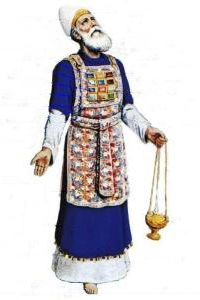
\includegraphics[width=50mm,scale=1.5]{Extras/Melchisedec.jpg}
\vspace{0.4in}  % Create a title for the document and write it in bold font
\LARGE{\textbf{\date}} % Again, do a line break
\linebreak 
% Create a subtitle \large{with Outlines, Statistics, Cross References, and Notes}
\vspace{0.5in}
\begin{flushleft}
\LARGE{Day \#29: Saturday, 29 January 2022 PLAIN   \\}\vspace{0.25in}
\LARGE{Exodus 34-36 Psalm 29 Proverb 29}
\end{flushleft}
\vspace{0.6in}
\bigskip

\normalsize{Xenia, Oh.\\}
\normalsize{created: \today}
\vspace{1.3in}

\end{flushright}
\end{titlepage}

%%%%%%%%%%%%
%%%%%%%%%%%%
%%%%%%%%%%%%

%\titleJE

\newpage 

\tableofcontents\hypertarget{TOC}{}
\listoffigures
\listoftables

\hyphenation{A-bim-e-lech bre-thren E-phra-im  Gib-e-o-nites Jer-u-sa-lem through-out Phil-i-stines The-o-phil-us Am-a-le-kites ven-geance Mesh-el-e-mi-ah onan-ism Phar-a-oh thoughts grev-ous-ness Hach-a-liah adul-ter-er Shad-rach}

%\fcolorbox{black}{bone}{TEXT}
%%%%%%%%%%%%%%%%% EXTRA COLORS
%%%%%%%%%%%%%%%%% EXTRA COLORS
%%%%%%%%%%%%%%%%% EXTRA COLORS
\definecolor{champagne}{rgb}{0.97,0.91,0.81}
\definecolor{bone}{rgb}{0.89,0.85,0.79}

\definecolor{ForestGreen}{rgb}{0.00,0.29,0.098}
\definecolor{GIVING}{cmyk}{1,0.0,0.72,.1}

\definecolor{MLPE}{cmyk}{1,1,0,.45}
\definecolor{SOCCER}{cmyk}{.77, 0, .42, .49}
\definecolor{PAYBILL}{cmyk}{0,0.83,0.76,0.07}
\definecolor{SERMON}{cmyk}{.14,.9,0,.30} % aka seance \href{http://www.flatuicolorpicker.com/purple-cmyk-color-model/}{seance}
\definecolor{BIBLE}{cmyk}{0,.17,.74,.17}
\definecolor{WORKBLUE}{cmyk}{1, .5, 0, .6}
\definecolor{myOrange}{cmyk}{0, .4, .98, .03}
\definecolor{myTan}{cmyk}{0.0,.07,.17,.10}
\definecolor{myRed}{cmyk}{0,1,1,0}
\definecolor{myWhite}{cmyk}{0,0,0,0}
\definecolor{BLUESoD}{cmyk}{.97,.84,0,.04}
\definecolor{WHITE}{cmyk}{0,0,0,0}
\definecolor{OLDGOLD}{cmyk}{0.05,0.3,1.00,0}
\definecolor{CASTLETON}{cmyk}{1,0,0.31,0.66}
\definecolor{cadmiumgreen}{rgb}{0.0, 0.42, 0.24}
\definecolor{jungle}{rgb}{0.203,0.4882,0.1718}
\definecolor{MYGOLD}{rgb}{1,.84,0}

\definecolor{MYLIGHTGRAY}{rgb}{.85,.85,.85}

\definecolor{codegreen}{rgb}{0,0.6,0}
\definecolor{codegray}{rgb}{0.5,0.5,0.5}
\definecolor{codepurple}{rgb}{0.58,0,0.82}
\definecolor{backcolour}{rgb}{0.95,0.95,0.92}



\mdfdefinestyle{MyFrame}{%
    linecolor=blue,
    outerlinewidth=2pt,
    roundcorner=5pt,
    innertopmargin=\baselineskip,
    innerbottommargin=\baselineskip,
    innerrightmargin=10pt,
    innerleftmargin=10pt,
    backgroundcolor=gray!25!white}


\mdfdefinestyle{MyFrame2}{%
    linecolor=black,
    outerlinewidth=2pt,
    roundcorner=5pt,
    innertopmargin=\baselineskip,
    innerbottommargin=\baselineskip,
    innerrightmargin=10pt,
    innerleftmargin=10pt,
    backgroundcolor=yellow!25!white}



%%%%%
%% for PFTTIS list
%%%%%

%%% And Joseph said unto
\index[PFTTIS]{And Joseph said unto!Genesis!Gen 40:008}
\index[PFTTIS]{And Joseph said unto!Genesis!Gen 40:012}
\index[PFTTIS]{And Joseph said unto!Genesis!Gen 41:025}
\index[PFTTIS]{And Joseph said unto!Genesis!Gen 42:014}
\index[PFTTIS]{And Joseph said unto!Genesis!Gen 42:018}
\index[PFTTIS]{And Joseph said unto!Genesis!Gen 44:015}
\index[PFTTIS]{And Joseph said unto!Genesis!Gen 45:003}
\index[PFTTIS]{And Joseph said unto!Genesis!Gen 45:004}
\index[PFTTIS]{And Joseph said unto!Genesis!Gen 46:031}
\index[PFTTIS]{And Joseph said unto!Genesis!Gen 48:009}
\index[PFTTIS]{And Joseph said unto!Genesis!Gen 48:018}
\index[PFTTIS]{And Joseph said unto!Genesis!Gen 50:019}
\index[PFTTIS]{And Joseph said unto!Genesis!Gen 50:024}


%%% a shadow
\index[PFTTIS]{a shadow!1Chronicles!1Chr 029:15}
\index[PFTTIS]{a shadow!Job!Job 008:09}
\index[PFTTIS]{a shadow!Job!Job 014:02}
\index[PFTTIS]{a shadow!Job!Job 017:07}
\index[PFTTIS]{a shadow!Psalm!Psa 102:011}
\index[PFTTIS]{a shadow!Psalm!Psa 144:004}
\index[PFTTIS]{a shadow!Ecclesiastes!Eccl 006:012}
\index[PFTTIS]{a shadow!Ecclesiastes!Eccl 008:013}
\index[PFTTIS]{a shadow!Isaiah!Isa 04:006}
\index[PFTTIS]{a shadow!Isaiah!Isa 25:004}
\index[PFTTIS]{a shadow!Jonah!Jnh 04:06}
\index[PFTTIS]{a shadow!Colossians!Col 02:017}
\index[PFTTIS]{a shadow!Hebews!Heb 10:001}

%%% blessed is the man
\index[PFTTIS]{blessed is the man!Psalm!Psa 001:001}
\index[PFTTIS]{blessed is the man!Psalm!Psa 032:002}
\index[PFTTIS]{blessed is the man!Psalm!Psa 034:008}
\index[PFTTIS]{blessed is the man!Psalm!Psa 065:004}
\index[PFTTIS]{blessed is the man!Psalm!Psa 084:005}
\index[PFTTIS]{blessed is the man!Psalm!Psa 084:012}
\index[PFTTIS]{blessed is the man!Psalm!Psa 094:012}
\index[PFTTIS]{blessed is the man!Psalm!Psa 112:001}
\index[PFTTIS]{blessed is the man!Proverbs!Pro 008:034}
\index[PFTTIS]{blessed is the man!Isaiah!Isa 056:002}
\index[PFTTIS]{blessed is the man!Jeremiah!Jer 017:007}
\index[PFTTIS]{blessed is the man!Romans!Rom 004:008}
\index[PFTTIS]{blessed is the man!James!Jam 001:012}


%%% carry them
\index[PFTTIS]{carry them!Leviticus!Lev 14:045}
\index[PFTTIS]{carry them!Numbers!Num 11:012}
\index[PFTTIS]{carry them!Joshua!Jsh 04:003}
\index[PFTTIS]{carry them!1Samuel!1Sam 20:040}
\index[PFTTIS]{carry them!1Kings!1Kng 08:046}
\index[PFTTIS]{carry them!2Chronicles!2Chr 06:036}
\index[PFTTIS]{carry them!Ezra!Ezra 05:015}
\index[PFTTIS]{carry them!Isaiah!Isa 40:011}
\index[PFTTIS]{carry them!Isaiah!Isa 41:016}
\index[PFTTIS]{carry them!Isaiah!Isa 57:013}
\index[PFTTIS]{carry them!Jeremiah!Jer 20:004}
\index[PFTTIS]{carry them!Jeremiah!Jer 20:005}
\index[PFTTIS]{carry them!Jeremiah!Jer 43:012}


\index[PFTTIS]{good tidings!2Samuel!2Sam 18:027}
\index[PFTTIS]{good tidings!1Kings!1Ki 01:042}
\index[PFTTIS]{good tidings!2Kings!2Ki 07:009 (2x)}
\index[PFTTIS]{good tidings!Isaiah!Isa 40:009 (2x)}
\index[PFTTIS]{good tidings!Isaiah!Isa 41:007}
\index[PFTTIS]{good tidings!Isaiah!Isa 52:007}
\index[PFTTIS]{good tidings!Isaiah!Isa 61:001}
\index[PFTTIS]{good tidings!Nahum!Nah 01:005}
\index[PFTTIS]{good tidings!Luke!Lk 02:010}
\index[PFTTIS]{good tidings!1Thessalonians!1Thess 03:006}


%%% dead body
\index[PFTTIS]{dead body!Leviticus!Lev 21:011}
\index[PFTTIS]{dead body!Numbers!Num 06:006}
\index[PFTTIS]{dead body!Numbers!Num 09:006}
\index[PFTTIS]{dead body!Numbers!Num 09:007}
\index[PFTTIS]{dead body!Numbers!Num 09:010}
\index[PFTTIS]{dead body!Numbers!Num 09:011}
\index[PFTTIS]{dead body!Numbers!Num 09:013}
\index[PFTTIS]{dead body!Numbers!Num 09:016}
\index[PFTTIS]{dead body!2Kings!2Ki 08:005}
\index[PFTTIS]{dead body!Isaiah!Isa 26:019}
\index[PFTTIS]{dead body!Jeremiah!Jer 26:023}
\index[PFTTIS]{dead body!Jeremiah!Jer 36:030}
\index[PFTTIS]{dead body!Haggai!Hag 02:013}

%%% great sea
\index[PFTTIS]{great sea!Numbers!Num 34:006}
\index[PFTTIS]{great sea!Numbers!Num 34:007}
\index[PFTTIS]{great sea!Joshua!Jos 01:004}
\index[PFTTIS]{great sea!Joshua!Jos 09:001}
\index[PFTTIS]{great sea!Joshua!Jos 15:012}
\index[PFTTIS]{great sea!Joshua!Jos 15:047}
\index[PFTTIS]{great sea!Joshua!Jos 23:004}
\index[PFTTIS]{great sea!Ezekiel!Eze 47:010}
\index[PFTTIS]{great sea!Ezekiel!Eze 47:015}
\index[PFTTIS]{great sea!Ezekiel!Eze 47:019}
\index[PFTTIS]{great sea!Ezekiel!Eze 47:020}
\index[PFTTIS]{great sea!Ezekiel!Eze 48:028}
\index[PFTTIS]{great sea!Daniel!Dan 07:002}


%%% have forsaken me
\index[PFTTIS]{have forsaken me!Judges!Jdg 10:013}
\index[PFTTIS]{have forsaken me!1Samuel!1Sam 08:008}
\index[PFTTIS]{have forsaken me!1Kings!1Ki 11:033}
\index[PFTTIS]{have forsaken me!2Kings!2Ki 22:017}
\index[PFTTIS]{have forsaken me!2Chronicles!2Chr 12:005}
\index[PFTTIS]{have forsaken me!2Chronicles!2Chr 34:025}
\index[PFTTIS]{have forsaken me!Jeremiah!Jer 01:016}
\index[PFTTIS]{have forsaken me!Jeremiah!Jer 02:013}
\index[PFTTIS]{have forsaken me!Jeremiah!Jer 05:007}
\index[PFTTIS]{have forsaken me!Jeremiah!Jer 05:019}
\index[PFTTIS]{have forsaken me!Jeremiah!Jer 16:011 (2x)}
\index[PFTTIS]{have forsaken me!Jeremiah!Jer 19:004}

%%% no king
\index[PFTTIS]{no king!Judges!Jdg 17:06}
\index[PFTTIS]{no king!Judges!Jdg 18:01}
\index[PFTTIS]{no king!Judges!Jdg 19:01}
\index[PFTTIS]{no king!Judges!Jdg 21:25}
\index[PFTTIS]{no king!1Kings!1Ki 22:47}
\index[PFTTIS]{no king!2Kings!2Ki 23:25}
\index[PFTTIS]{no king!Nehemiah!Neh 13:26}
\index[PFTTIS]{no king!Psalms!Psa 033:016}
\index[PFTTIS]{no king!Proverbs!Pro 30:27}
\index[PFTTIS]{no king!Daniel!Dan 02:10}
\index[PFTTIS]{no king!Hosea!Hos 10:03}
\index[PFTTIS]{no king!Micah!Mic 04:09}
\index[PFTTIS]{no king!John!Jhn 19:15}


%%% rebellious house
\index[PFTTIS]{rebellious house!Exodus!Exo 02:005}
\index[PFTTIS]{rebellious house!Exodus!Exo 02:006}
\index[PFTTIS]{rebellious house!Exodus!Exo 02:008}
\index[PFTTIS]{rebellious house!Exodus!Exo 03:009}
\index[PFTTIS]{rebellious house!Exodus!Exo 03:026}
\index[PFTTIS]{rebellious house!Exodus!Exo 03:027}
\index[PFTTIS]{rebellious house!Exodus!Exo 12:002 (2x)}
\index[PFTTIS]{rebellious house!Exodus!Exo 12:003}
\index[PFTTIS]{rebellious house!Exodus!Exo 12:009}
\index[PFTTIS]{rebellious house!Exodus!Exo 12:025}
\index[PFTTIS]{rebellious house!Exodus!Exo 17:012}
\index[PFTTIS]{rebellious house!Exodus!Exo 24:003}

%%% seek him
\index[PFTTIS]{seek him!Deuteronomy!Deu 04:029}\index[PFTTIS]{seek him!1Samuel!1Sam 23:025}
\index[PFTTIS]{seek him!1Chronicles!1Chr 28:009}
\index[PFTTIS]{seek him!2Chronicles!1Chr 15:002}
\index[PFTTIS]{seek him!Ezra!Ezr 08:022}
\index[PFTTIS]{seek him!Psalms!Psa 022:026}
\index[PFTTIS]{seek him!Psalms!Psa 024:006}
\index[PFTTIS]{seek him!Psalms!Psa 119:002}
\index[PFTTIS]{seek him!SoS!SoS 03:002}
\index[PFTTIS]{seek him!SoS!SoS 06:001}
\index[PFTTIS]{seek him!Hosea!Hos 07:010}
\index[PFTTIS]{seek him!Amos!Amo 05:008}
\index[PFTTIS]{seek him!Hebrews!Heb 11:0063}


%%% seek ye
\index[PFTTIS]{seek ye!Isaiah!Isa 34:016}
\index[PFTTIS]{seek ye!Isaiah!Isa 45:019}
\index[PFTTIS]{seek ye!Isaiah!Isa 55:006}
\index[PFTTIS]{seek ye!Amos!Amos 5:004}
\index[PFTTIS]{seek ye!John!John 1:38}
\index[PFTTIS]{seek ye!John!John 18:4}
\index[PFTTIS]{seek ye!John!John 18:7}
\index[PFTTIS]{seek ye!Matthew!Matt 6:33}
\index[PFTTIS]{seek ye!Numbers!Num 16:10}
\index[PFTTIS]{seek ye!Luke!Luke 12:31}
\index[PFTTIS]{seek ye!Luke!Luke 24:5}
\index[PFTTIS]{seek ye!Psalm!Psa 27:8}
\index[PFTTIS]{seek ye!Zephaniah!Zeph 2:3}

%%% the uncircumcised
\index[PFTTIS]{the uncircumcised!Genesis!Gen 17:014}
\index[PFTTIS]{the uncircumcised!Judges!Jdg 14:003}
\index[PFTTIS]{the uncircumcised!Judges!Jdg 15:018}
\index[PFTTIS]{the uncircumcised!2Samuel!2Sam 01:020}
\index[PFTTIS]{the uncircumcised!Isaiah!Isa 02:001}
\index[PFTTIS]{the uncircumcised!Jeremiah!Jer 09:025}
\index[PFTTIS]{the uncircumcised!Ezekiel!Eze 28:010}
\index[PFTTIS]{the uncircumcised!Ezekiel!Eze 31:018}
\index[PFTTIS]{the uncircumcised!Ezekiel!Eze 32:019}
\index[PFTTIS]{the uncircumcised!Ezekiel!Eze 32:027}
\index[PFTTIS]{the uncircumcised!Ezekiel!Eze 32:028}
\index[PFTTIS]{the uncircumcised!Ezekiel!Eze 32:029}
\index[PFTTIS]{the uncircumcised!Ezekiel!Eze 32:032}

%%% worship him
\index[PFTTIS]{worship him!Psalms!Psa 97:007}
\index[PFTTIS]{worship him!Zephaniah!Zeph 02:011}
\index[PFTTIS]{worship him!Matthew!Matt 02:002}
\index[PFTTIS]{worship him!Matthew!Matt 02:008}
\index[PFTTIS]{worship him!John!John 04:023}
\index[PFTTIS]{worship him!John!John 04:024 (2x)} 
\index[PFTTIS]{worship him!Acts!Acts 17:023}
\index[PFTTIS]{worship him!Hebrews!Heb 01:006}
\index[PFTTIS]{worship him!Revelation!Rev 04:010}
\index[PFTTIS]{worship him!Revelation!Rev 13:008}
\index[PFTTIS]{worship him!Revelation!Rev 14:007}
\index[PFTTIS]{worship him!Revelation!Rev 19:010}


%%%%%
%% for PFTTIS list
%%%%%

%%% afflictions
\index[WFTTIS]{afflictions!Psalms!Psa 34:019}
\index[WFTTIS]{afflictions!Psalms!Psa 132:001}
\index[WFTTIS]{afflictions!Acts!Acts 07:010}
\index[WFTTIS]{afflictions!Acts!Acts 20:023}
\index[WFTTIS]{afflictions!2Corinthians!2Cor 06:004}
\index[WFTTIS]{afflictions!Colossians!Col 01:024}
\index[WFTTIS]{afflictions!1Thessalonians!1Thess 03:003}
\index[WFTTIS]{afflictions!2Timothy!2Tim 01:008}
\index[WFTTIS]{afflictions!2Timothy!2Tim 03:011}
\index[WFTTIS]{afflictions!2Timothy!2Tim 04:005}
\index[WFTTIS]{afflictions!Hebrews!Heb 10:032}
\index[WFTTIS]{afflictions!Hebrews!Heb 10:033}
\index[WFTTIS]{afflictions!1Peter!1Pet 05:009}

%%% acsend
\index[WFTTIS]{acsend!Joshua!Jos 06:05}
\index[WFTTIS]{acsend!Psalm!Psa 024:003}
\index[WFTTIS]{acsend!Psalm!Psa 135:007}
\index[WFTTIS]{acsend!Psalm!Psa 139:008}
\index[WFTTIS]{acsend!Isaiah!Isa 14:013}
\index[WFTTIS]{acsend!Isaiah!Isa 14:014}
\index[WFTTIS]{acsend!Jeremiah!Jer 10:013}
\index[WFTTIS]{acsend!Jeremiah!Jer 51:016}
\index[WFTTIS]{acsend!Ezekiel!Eze 38:009}
\index[WFTTIS]{acsend!John!John 06:062}
\index[WFTTIS]{acsend!John!John 20:017}
\index[WFTTIS]{acsend!Romans!Rom 10:006}
\index[WFTTIS]{acsend!Revelation!Rev 17:008}

%%% Assyrian
\index[WFTTIS]{Assyrian!Isaiah!Isa 10:005}
\index[WFTTIS]{Assyrian!Isaiah!Isa 10:024}
\index[WFTTIS]{Assyrian!Isaiah!Isa 14:025}
\index[WFTTIS]{Assyrian!Isaiah!Isa 19:023}
\index[WFTTIS]{Assyrian!Isaiah!Isa 23:013}
\index[WFTTIS]{Assyrian!Isaiah!Isa 30:031}
\index[WFTTIS]{Assyrian!Isaiah!Isa 31:008}
\index[WFTTIS]{Assyrian!Isaiah!Isa 52:004}
\index[WFTTIS]{Assyrian!Ezekiel!Eze 31:003}
\index[WFTTIS]{Assyrian!Hosea!Hos 05:013}
\index[WFTTIS]{Assyrian!Hosea!Hos 11:005}
\index[WFTTIS]{Assyrian!Micah!Hos 05:005}
\index[WFTTIS]{Assyrian!Micah!Hos 05:006}

%%% blot
\index[WFTTIS]{blot!Exodus!Exo 32:032}
\index[WFTTIS]{blot!Exodus!Exo 32:033}
\index[WFTTIS]{blot!Numbers!Num 05:026}
\index[WFTTIS]{blot!Deuteronomy!Deut 09:014}
\index[WFTTIS]{blot!Deuteronomy!Deut 25:019}
\index[WFTTIS]{blot!Deuteronomy!Deut 29:020}
\index[WFTTIS]{blot!2Kings!2Ki 14:027}
\index[WFTTIS]{blot!Job!Job 31:007}
\index[WFTTIS]{blot!Psalms!Psa 51:001}
\index[WFTTIS]{blot!Psalms!Psa 51:009}
\index[WFTTIS]{blot!Proverbs!Pro 09:007}
\index[WFTTIS]{blot!Jeremiah!Jer 18:023}
\index[WFTTIS]{blot!Revelation!Rev 03:005}


%%% chain
\index[WFTTIS]{chain!Genesis!Gen 41:042}
\index[WFTTIS]{chain!1Kings!1Ki 07:017}
\index[WFTTIS]{chain!Psalms!Psa 73:006}
\index[WFTTIS]{chain!SoS!Sos 04:009}
\index[WFTTIS]{chain!Lamentations!Lam 03:007}
\index[WFTTIS]{chain!Ezekiel!Eze 07:023}
\index[WFTTIS]{chain!Ezekiel!Eze 16:011}
\index[WFTTIS]{chain!Daniel!Dan 05:007}
\index[WFTTIS]{chain!Daniel!Dan 05:016}
\index[WFTTIS]{chain!Daniel!Dan 05:029}
\index[WFTTIS]{chain!Acts!Acts 28:020}
\index[WFTTIS]{chain!2Timothy!2Tim 01:016}
\index[WFTTIS]{chain!Revelation!Rev 20:001}


%%% controversy
\index[WFTTIS]{controversy!Deuteronomy!Deu 17:008}
\index[WFTTIS]{controversy!Deuteronomy!Deu 19:017}
\index[WFTTIS]{controversy!Deuteronomy!Deu 21:005}
\index[WFTTIS]{controversy!Deuteronomy!Deu 25:001}
\index[WFTTIS]{controversy!2Samuel!2Sam 15:002}
\index[WFTTIS]{controversy!Isaiah!Isa 34:008}
\index[WFTTIS]{controversy!Jeremiah!Jer 25:031}
\index[WFTTIS]{controversy!Ezekiel!Eze 44:024}
\index[WFTTIS]{controversy!Hosea!Hos 04:001}
\index[WFTTIS]{controversy!Hosea!Hos 12:002}
\index[WFTTIS]{controversy!Micah!Mic 06:002 (2x)}
\index[WFTTIS]{controversy!1Timothy!1Tim 03:016}


%%% Dagon/Dagon's
\index[WFTTIS]{Dagon!Judges!Jdg 16:023}
\index[WFTTIS]{Dagon!1Samuel!1Sam 05:002 (2x)}
\index[WFTTIS]{Dagon!1Samuel!1Sam 05:003 (2x)}
\index[WFTTIS]{Dagon!1Samuel!1Sam 05:004 (3x)}
\index[WFTTIS]{Dagon!1Samuel!1Sam 05:005 (3x)}
\index[WFTTIS]{Dagon!1Samuel!1Sam 05:007}
\index[WFTTIS]{Dagon!1Chronicles!1Chr 10:010}

%%% disobedient
\index[WFTTIS]{disobedient!1Kings!1Ki 13:026}
\index[WFTTIS]{disobedient!Nehemiah!Neh 09:026}
\index[WFTTIS]{disobedient!Luke!Luke 01:017}
\index[WFTTIS]{disobedient!Acts!Acts 26:019}
\index[WFTTIS]{disobedient!Romans!Rom 01:030}
\index[WFTTIS]{disobedient!Romans!Rom 10:021}
\index[WFTTIS]{disobedient!1Timothy!1Tim 01:009}
\index[WFTTIS]{disobedient!2Timothy!2Tim 03:002}
\index[WFTTIS]{disobedient!Titus!Titus 01:016}
\index[WFTTIS]{disobedient!Titus!Titus 03:003}
\index[WFTTIS]{disobedient!1Peter!1Pet 02:007}
\index[WFTTIS]{disobedient!1Peter!1Pet 02:008}
\index[WFTTIS]{disobedient!1Peter!1Pet 03:020}


%%% doubt
\index[WFTTIS]{doubt!Genesis!Gen 37:033}
\index[WFTTIS]{doubt!Deuteronomy!Deu 28:066}
\index[WFTTIS]{doubt!Job!Job 12:002}
\index[WFTTIS]{doubt!Matthew!Matt 14:031}
\index[WFTTIS]{doubt!Matthew!Matt 21:021}
\index[WFTTIS]{doubt!Mark!Mk 11:023}
\index[WFTTIS]{doubt!Luke!Lk 11:020}
\index[WFTTIS]{doubt!John!Jhn 10:024}
\index[WFTTIS]{doubt!Acts!Acts 02:012}
\index[WFTTIS]{doubt!Acts!Acts 28:004}
\index[WFTTIS]{doubt!1Corinthians!1Cor 09:010}
\index[WFTTIS]{doubt!Galatians!Gal 04:020}
\index[WFTTIS]{doubt!1John!1Jhn 02:019}


%%% dungeon
\index[WFTTIS]{dungeon!Genesis!Gen 40:015}
\index[WFTTIS]{dungeon!Genesis!Gen 41:014}
\index[WFTTIS]{dungeon!Exodus!Exo 12:029}
\index[WFTTIS]{dungeon!Jeremiah!Jer 37:016}
\index[WFTTIS]{dungeon!Jeremiah!Jer 38:006 (2x)}
\index[WFTTIS]{dungeon!Jeremiah!Jer 38:007}
\index[WFTTIS]{dungeon!Jeremiah!Jer 38:009}
\index[WFTTIS]{dungeon!Jeremiah!Jer 38:010}
\index[WFTTIS]{dungeon!Jeremiah!Jer 38:011}
\index[WFTTIS]{dungeon!Jeremiah!Jer 38:013}
\index[WFTTIS]{dungeon!Lamentations!Lam 03:053}
\index[WFTTIS]{dungeon!Lamentations!Lam 03:055}


%%% error
\index[WFTTIS]{error!2Samuel!2Sam 06:007}
\index[WFTTIS]{error!Job!Job 19:004}
\index[WFTTIS]{error!Ecclesiastes!Ecc 05:006}
\index[WFTTIS]{error!Ecclesiastes!Ecc 10:005}
\index[WFTTIS]{error!Isaiah!Isa 32:006}
\index[WFTTIS]{error!Daniel!Dan 06:004}
\index[WFTTIS]{error!Matthew!Matt 27:064}
\index[WFTTIS]{error!Romans!Rom 01:027}
\index[WFTTIS]{error!James!Jam 05:020}
\index[WFTTIS]{error!2Peter!2Pet 02:018}
\index[WFTTIS]{error!2Peter!2Pet 03:017}
\index[WFTTIS]{error!1John!1Jn 04:006}
\index[WFTTIS]{error!Jude!Jude 01:011}

%%% fourish
\index[WFTTIS]{fourish!Psalms!Psa 072:007}
\index[WFTTIS]{fourish!Psalms!Psa 072:016}
\index[WFTTIS]{fourish!Psalms!Psa 092:007}
\index[WFTTIS]{fourish!Psalms!Psa 092:012}
\index[WFTTIS]{fourish!Psalms!Psa 092:013}
\index[WFTTIS]{fourish!Psalms!Psa 132:018}
\index[WFTTIS]{fourish!Proverbs!Pro 11:28}
\index[WFTTIS]{fourish!Proverbs!Pro 14:11}
\index[WFTTIS]{fourish!Ecclesiastes!Ecc 12:05}
\index[WFTTIS]{fourish!SongOfSolomon!SOS 07:12}
\index[WFTTIS]{fourish!Isaiah!Isa 17:11}
\index[WFTTIS]{fourish!Isaiah!Isa 66:14}
\index[WFTTIS]{fourish!Ezekiel!Eze 17:24}




%%% giants
\index[WFTTIS]{giants!Genesis!Gen 06:004}
\index[WFTTIS]{giants!Numbers!Num 13:033}
\index[WFTTIS]{giants!Deuteronomy!Deut 02:011}
\index[WFTTIS]{giants!Deuteronomy!Deut 02:021}
\index[WFTTIS]{giants!Deuteronomy!Deut 03:011}
\index[WFTTIS]{giants!Deuteronomy!Deut 03:013}
\index[WFTTIS]{giants!Joshua!Josh 12:004}
\index[WFTTIS]{giants!Joshua!Josh 13:012}
\index[WFTTIS]{giants!Joshua!Josh 15:008}
\index[WFTTIS]{giants!Joshua!Josh 17:015}
\index[WFTTIS]{giants!Joshua!Josh 16:016}

%%% good man
\index[WFTTIS]{good man!2 Samuel!2Sa 18:27}
%(1) Psalms 37:23 [5]
%(1) Psalms 112:5 [2]
%(1) Proverbs 12:2 [2]
%(1) Proverbs 13:22 [2]
%(1) Proverbs 14:14 [14]
%(1) Micah 7:2 [2]
%(1) Matthew 12:35 [2]
%(1) Luke 6:45 [2]
%(1) Luke 23:50 [15]
%(1) John 7:12 [17]
%(1) Acts 11:24 [5]
%(1) Romans 5:7 [14]

%%% Hinnom
\index[WFTTIS]{Hinnom!Joshua!Jsh 15:008}
\index[WFTTIS]{Hinnom!Joshua!Jsh 18:016}
\index[WFTTIS]{Hinnom!2Kings!2Ki 23:010}
\index[WFTTIS]{Hinnom!2Chronicles!2Chr 28:003}
\index[WFTTIS]{Hinnom!2Chronicles!2Chr 33:006}
\index[WFTTIS]{Hinnom!Nehemiah!Neh 11:030}
\index[WFTTIS]{Hinnom!Jeremiah!Jer 07:031}
\index[WFTTIS]{Hinnom!Jeremiah!Jer 07:032}
\index[WFTTIS]{Hinnom!Jeremiah!Jer 19:002}
\index[WFTTIS]{Hinnom!Jeremiah!Jer 19:006}
\index[WFTTIS]{Hinnom!Jeremiah!Jer 32:035}

%%% inclined
\index[WFTTIS]{inclined!Judges!Jdg 09:003}
\index[WFTTIS]{inclined!Psalms!Psa 040:001}
\index[WFTTIS]{inclined!Psalms!Psa 116:002}
\index[WFTTIS]{inclined!Psalms!Psa 119:112}
\index[WFTTIS]{inclined!Proverbs!Pro 05:13}
\index[WFTTIS]{inclined!Jeremiah!Jer 07:24}
\index[WFTTIS]{inclined!Jeremiah!Jer 07:26}
\index[WFTTIS]{inclined!Jeremiah!Jer 11:08}
\index[WFTTIS]{inclined!Jeremiah!Jer 17:23}
\index[WFTTIS]{inclined!Jeremiah!Jer 25:04}
\index[WFTTIS]{inclined!Jeremiah!Jer 34:14}
\index[WFTTIS]{inclined!Jeremiah!Jer 35:15}
\index[WFTTIS]{inclined!Jeremiah!Jer 44:05}


%%% laughed
\index[WFTTIS]{laughed!Genesis!Gen 17:017}
\index[WFTTIS]{laughed!Genesis!Gen 18:012}
\index[WFTTIS]{laughed!Genesis!Gen 18:015}
\index[WFTTIS]{laughed!2Kings!2Ki 19:021}
\index[WFTTIS]{laughed!2Chronicles!2Chr 30:010}
\index[WFTTIS]{laughed!Nehemiah!Neh 02:019}
\index[WFTTIS]{laughed!Job!Job 12:004}
\index[WFTTIS]{laughed!Job!Job 29:024}
\index[WFTTIS]{laughed!Isaiah!Isa 37:022}
\index[WFTTIS]{laughed!Ezekiel!Ezek 23:032}
\index[WFTTIS]{laughed!Matthew!Matt 09:024}
\index[WFTTIS]{laughed!Mark!Mk 05:040}
\index[WFTTIS]{laughed!Luke!Lk 08:053}

%%% liar
\index[WFTTIS]{liar!Job!Job 24:025}
\index[WFTTIS]{liar!Proverbs!Pro 17:004}
\index[WFTTIS]{liar!Proverbs!Pro 19:022}
\index[WFTTIS]{liar!Proverbs!Pro 30:006}
\index[WFTTIS]{liar!Jeremiah!Jer 15:018}
\index[WFTTIS]{liar!John!Jhn 08:044}
\index[WFTTIS]{liar!John!Jhn 08:055}
\index[WFTTIS]{liar!Romans!Rom 03:004}
\index[WFTTIS]{liar!1John!1Jhn 01:010}
\index[WFTTIS]{liar!1John!1Jhn 02:004}
\index[WFTTIS]{liar!1John!1Jhn 02:022}
\index[WFTTIS]{liar!1John!1Jhn 04:020}
\index[WFTTIS]{liar!1John!1Jhn 05:010}

%%% palsy
\index[WFTTIS]{palsy!Matthew!Matt 04:024}
\index[WFTTIS]{palsy!Matthew!Matt 08:006}
\index[WFTTIS]{palsy!Matthew!Matt 09:002}
\index[WFTTIS]{palsy!Matthew!Matt 09:006}
\index[WFTTIS]{palsy!Mark!Mk 02:003}
\index[WFTTIS]{palsy!Mark!Mk 02:004}
\index[WFTTIS]{palsy!Mark!Mk 02:005}
\index[WFTTIS]{palsy!Mark!Mk 02:009}
\index[WFTTIS]{palsy!Mark!Mk 02:010}
\index[WFTTIS]{palsy!Luke!Lk 05:018}
\index[WFTTIS]{palsy!Luke!Lk 05:024}
\index[WFTTIS]{palsy!Acts!Acts 09:033}

%%% Profitable
\index[WFTTIS]{profitable!Job!Job 22:002 (2x)}
\index[WFTTIS]{profitable!Ecclesiastes!Ecc 10:010}
\index[WFTTIS]{profitable!Isaiah!Isa 44:010}
\index[WFTTIS]{profitable!Jeremiah!Jer 13:007}
\index[WFTTIS]{profitable!Matthew!Matt 05:029}
\index[WFTTIS]{profitable!Matthew!Matt 05:030}
\index[WFTTIS]{profitable!Acts!Acts 20:020}
\index[WFTTIS]{profitable!1Timothy!1Tim 04:008}
\index[WFTTIS]{profitable!2Timothy!2Tim 03:016}
\index[WFTTIS]{profitable!2Timothy!2Tim 04:011}
\index[WFTTIS]{profitable!Titus!Titus 03:008}
\index[WFTTIS]{profitable!Philemon!Phlm 01:011}

%%% Rechab
\index[WFTTIS]{Rechab!2Samuel!2Sam 04:002}
\index[WFTTIS]{Rechab!2Samuel!2Sam 04:005}
\index[WFTTIS]{Rechab!2Samuel!2Sam 04:006}
\index[WFTTIS]{Rechab!2Samuel!2Sam 04:009}
\index[WFTTIS]{Rechab!2KIngs!2Ki 10:015}
\index[WFTTIS]{Rechab!2KIngs!2Ki 10:023}
\index[WFTTIS]{Rechab!1Chronicles!1Chr 02:055}
\index[WFTTIS]{Rechab!Nehemiah!Neh 03:014}
\index[WFTTIS]{Rechab!Jeremiah!Jer 35:006}
\index[WFTTIS]{Rechab!Jeremiah!Jer 35:008}
\index[WFTTIS]{Rechab!Jeremiah!Jer 35:014}
\index[WFTTIS]{Rechab!Jeremiah!Jer 35:016}
\index[WFTTIS]{Rechab!Jeremiah!Jer 35:019}

%%% serpents
\index[WFTTIS]{serpents!Exodus!Exo 07:012}
\index[WFTTIS]{serpents!Numbers!Num 21:006}
\index[WFTTIS]{serpents!Numbers!Num 21:007}
\index[WFTTIS]{serpents!Deuteronomy!Deu 08:015}
\index[WFTTIS]{serpents!Deuteronomy!Deu 32:024}
\index[WFTTIS]{serpents!Jeremiah!Jer 08:017}
\index[WFTTIS]{serpents!Matthew!Matt 10:016}
\index[WFTTIS]{serpents!Matthew!Matt 23:033}
\index[WFTTIS]{serpents!Mark!Mk 16:018}
\index[WFTTIS]{serpents!Luke!Lk 10:019}
\index[WFTTIS]{serpents!1Corinthians!1Cor 10:009}
\index[WFTTIS]{serpents!James!Jas 03:007}
\index[WFTTIS]{serpents!Revelation!Rev 09:019}

%%% short
\index[WFTTIS]{short!Numbers!Num 11:023}
\index[WFTTIS]{short!2Kings!2Ki 10:032}
\index[WFTTIS]{short!Job!Job 17:012}
\index[WFTTIS]{short!Job!Job 20:005}
\index[WFTTIS]{short!Psalms!Psa 89:047}
\index[WFTTIS]{short!Romans!Rom 03:023}
\index[WFTTIS]{short!Romans!Rom 09:028  (2x)}
\index[WFTTIS]{short!1Corinthians!1Cor 07:029}
\index[WFTTIS]{short!1Thessalonians!1Thess 02:017}
\index[WFTTIS]{short!Hebrews!Heb 04:001}
\index[WFTTIS]{short!Revelation!Rev 12:012}
\index[WFTTIS]{short!Revelation!Rev 17:010}

%%% smiteth
\index[WFTTIS]{smiteth!Exodus!Exo 21:012}
\index[WFTTIS]{smiteth!Exodus!Exo 21:15}
\index[WFTTIS]{smiteth!Deuteronomy!Dt 25:11}
\index[WFTTIS]{smiteth!Deuteronomy!Dt 27:24}
\index[WFTTIS]{smiteth!Joshua!Jsh 15:16}
\index[WFTTIS]{smiteth!Judges!Jdg 15:16}
\index[WFTTIS]{smiteth!2 Samuel!2Sa 05:08}
\index[WFTTIS]{smiteth!1Chronicles!1Chr 11:06}
\index[WFTTIS]{smiteth!Job!1Chr 26:12}
\index[WFTTIS]{smiteth!Isaiah!Isa 09:13}
\index[WFTTIS]{smiteth!Lamentations!Lam 03:30}
\index[WFTTIS]{smiteth!Ezekiel!Eze 07:09}
\index[WFTTIS]{smiteth!Luke!Lk 06:29}



%%% vanities
\index[WFTTIS]{vanities!Deuteronomy!Deut 21:021}
\index[WFTTIS]{vanities!1Kings!1Ki 16:013}
\index[WFTTIS]{vanities!1Kings!1Ki 16:026}
\index[WFTTIS]{vanities!Psalms!Psa 031:006}
\index[WFTTIS]{vanities!Ecclesiastes!Ecc 01:002 (2x)}
\index[WFTTIS]{vanities!Ecclesiastes!Ecc 05:007}
\index[WFTTIS]{vanities!Ecclesiastes!Ecc 12:008}
\index[WFTTIS]{vanities!Jeremiah!Jer 08:019}
\index[WFTTIS]{vanities!Jeremiah!Jer 10:008}
\index[WFTTIS]{vanities!Jeremiah!Jer 14:022}
\index[WFTTIS]{vanities!Jonah!Jnh 02:008}
\index[WFTTIS]{vanities!Acts!Acts 14:015}



%%%%%
%% for PFTTIS list
%%%%%

%%% worm
\index[WFITV]{worm!Exodus!Exo 16:024}
\index[WFITV]{worm!Job!Job 17:014}
\index[WFITV]{worm!Job!Job 24:029}
\index[WFITV]{worm!Job!Job 25:005 (2x)}
\index[WFITV]{worm!Psalms!Psa 022:006}
\index[WFITV]{worm!Isaiah!Isa 14:011}
\index[WFITV]{worm!Isaiah!Isa 41:014}
\index[WFITV]{worm!Isaiah!Isa 51:008}
\index[WFITV]{worm!Isaiah!Isa 66:024}
\index[WFITV]{worm!Jonah!Jnh 04:007}
\index[WFITV]{worm!Mark!Mk 09:044}
\index[WFITV]{worm!Mark!Mk 09:046}
\index[WFITV]{worm!Mark!Mk 09:048}


%\subsubsection{Title}
%\textbf{Introduction:} Isaiah 46 
%\index[speaker]{Speaker!Isaiah 49 (Title}
%\index[series]{Book (Speaker)!IPassage (Title)}
%\index[date]{2017/07/09!Isaiah 49 (Title)}
%\begin{compactenum}[I.]
%    \item  \textbf{Point} \index[scripture]{Isaiah!IPassage} (IPassage)
%\end{compactenum}




  

\chapter{Today's Readings}

\normalsize
 
\begin{center}
\begin{longtable}{|p{0.45in}|p{0.25in}|p{0.4in}|p{2.8in}|c|c|}
\caption[Today's Chapters]{Today's Chapters}\label{table:Today's Chapters} \\
\hline 
\multicolumn{1}{|c|}{\textbf{Chap}} & 
\multicolumn{1}{|c|}{\textbf{\#}} & 
\multicolumn{1}{|c|}{\textbf{Rvrs} } & 
\multicolumn{1}{|c|}{\textbf{address numerics}} & 
\multicolumn{1}{|c|}{\textbf{Vss}} & 
\multicolumn{1}{|c|}{\textbf{wds}}  \\ 
\hline 
\endfirsthead

 
\multicolumn{6}{c}
{{\bfseries \tablename\ \thetable{} -- continued from previous page}} \\  
\hline \multicolumn{1}{|c|}{\textbf{Chap}} & \multicolumn{1}{|c|}{\textbf{\#}} & \multicolumn{1}{|c|}{\textbf{Rev}} & \multicolumn{1}{|c|}{\textbf{addr Num}} & \multicolumn{1}{|c|}{\textbf{Verses}} & \multicolumn{1}{|c|}{\textbf{words}}  \\ \hline \endhead
 
%\hline \multicolumn{6}{|r|}{{Continued}} \\ \hline
\endfoot 
%Exo 20 & 70 & 1120 & 70 = 2 * 5 * 7; 1120 = 2 * 2 * 2 * 2 * 2 * 5 * 7 & 26 & 561 \\ \hline
%Exo 21 & 71 & 1119 & 71 is prime; 1119 = 3 * 373 & 36 & 893 \\ \hline \hline
%Exo 22 & 72 & 1118 &72 = 2 * 2 * 3 * 3; 1118 = 2 * 13 * 17 & 31 & 790 \\ \hline
%Exo 23 & 73 & 1117 & 73 is prime; 1117 is & 33 & 827 \\ \hline
%Exo 24 & 74 & 1116 & 74 = 2 * 37; 1116 = 2 8 2 * 3 * 3 * 31 & 18 & 492 \\ \hline \hline
%Exo 25 & 75 & 1115 & 75 = 3 * 5 * 5; 1115 = 5 * 223 & 40 & 926 \\ \hline
%Exo 26 & 76 & 1114 & 76 = 2 * 2 * 19; 1114 = 2 * 557 & 37 & 937 \\ \hline
%Exo 27 & 77 & 1113 & 77 = 7 * 11; 1113 = 3 * 7 * 53 & 18 & 492 \\ \hline \hline
%Exo 28 & 78 & 1112 & 78 = 2 * 3 * 13; 1112 = 2 * 2 * 2 * 139 & 43 & 1235 \\ \hline
%Exo 28 & 79 & 1111 & 79 is prime; 1111 = 11 * 101 & 46 & 1341 \\ \hline
%Exo 30 & 80 & 1110 & 80 = 2 * 2 * 2 * 2 * 5; 1110 = 2 * 3 * 5 * 37 & 38 & 970 \\ \hline \hline
%Exo 31 & 81 & 1109 & 81 = 3 * 3 * 3 * 3; 1109 is prime & 18 & 438 \\ \hline
%Exo 32 & 82 & 1108 & 82 = 1 * 41; 1108 = 2 * 2 * 277 & 35 & 1093 \\ \hline
%Exo 33 & 83 & 1107 & 83 is prime; 1107 = 3 * 3 * 3 * 41  & 23 & 710 \\ \hline \hline
Exo 34 & 84 & 1106 & 84 = 2 * 2 * 3 * 7; 1106 = 3 * 7 * 79 & 18 & 438 \\ \hline
Exo 35 & 85 & 1105 & 85 = 5 * 17; 1105 = 5 * 13 * 17 & 35 & 1093 \\ \hline
Exo 36 & 86 & 1104 & 86 = 2 * 43; 1104 = 2 * 2 * 2 * 2 * 3 * 23 & 23 & 710 \\ \hline \hline

%Psa 23 & 501 & 690 & 501 is prime; 690 = 2 * 3 * 5 * 23 & 31 & 246 \\ \hline \hline
%Psa 24 & 502 & 689 & 502 = 2 * 251 ; 689  = 13 * 53 & 10 & 178 \\ \hline \hline
%Psa 25 & 503 & 688 &  503 is prime ; 688  = 2 * 2 * 2 * 2 * 43 & 22 & 342 \\ \hline 
%Psa 27 & 504 & 687 &  504 = 2 * 2 * 2 * 3 * 3 * 7 ; 687  = 3 * 229 & 14 & 340 \\ \hline \hline
%Psa 28 & 505 & 686 &  505 = 5 * 101 ; 686  = 2 * 7 * 7 * 7 & 9 & 201 \\ \hline \hline
Psa 29 & 506 & 685 &  506 = 2 * 11 * 23 ; 685 = 5 * 137 & 11 & 179 \\ \hline \hline

%Pro 23 & 651 & 539 & 651 = 3 * 7 * 31; 539 = 7 * 7 * 11 & 35 & 566 \\ \hline \hline
%Pro 24 & 652 & 538 & 652 = 2 * 2 * 163; 538 = 2 * 269 & 34 & 580 \\ \hline \hline
%Pro 25 & 653 & 537 & 653 is prime; 537 = 3 * 179 & 28 & 522 \\ \hline \hline
%Pro 27 & 654 & 536 & 654 = 2 * 3 * 109; 536 = 2 * 2 * 2 * 67 & 23 & 460 \\ \hline 
%Pro 28 & 655 & 535 & 655 = 5 * 131; 535 = 5 * 107& 28 & 527 \\ \hline 
Pro 29 & 656 & 534 & 656 = 2 * 2 * 2 * 2 * 41; 534 = 2 * 3 * 89 & 27 & 425 \\ \hline 

\end{longtable}
\end{center}

%%%%%%%%%%%%%%%%%%%%%%%%%%%%%%%%%%%%%%%%%%%%
%%%%%%%%%%%%%%%%%%%%%%%%%%%%%%%%%%%%%%%%%%%%

\begin{center}
\begin{longtable}{|p{0.7in}|p{3.8in}|}
\caption[Today's Chapter Summaries]{Today's Chapter Summaries}\label{table:Today's Chapter Summaries} \\
\hline \multicolumn{1}{|c|}{\textbf{Chap}} & \multicolumn{1}{|c|}{\textbf{comments}}  \\ \hline 
\endfirsthead
 
\multicolumn{2}{c}
{{\bfseries \tablename\ \thetable{} -- continued from previous page}} \\  
\hline \multicolumn{1}{|c|}{\textbf{Chap}} & \multicolumn{1}{|c|}{\textbf{comments}}  \\ \hline 
 \\ \hline 
\endhead
 
%\hline \multicolumn{2}{|r|}{{}} \\ \hline
\endfoot 
Exo 34 & Moses made new tablets for the law. The LORD spoke to him and made a covenant with Israel. When Moses returned his face was shining.  \\ \hline
Exo 35 & Moses told the Israelites to keep the Sabbath. He called for craftsmen to make the tabernacle. The people gave gifts for the work. \\ \hline
Exo 36 & The people gave more than enough. The craftsmen made the curtains. Bezalel made the curtains, the boards, the veil and the pillars. \\ \hline

Psa 29 &  The people gave more than enough. The craftsmen made the curtains. Bezalel made the curtains, the boards, the veil and the pillars. \\ \hline
Prov 29 & By justice a king builds up the land. Whether a fool rages or laughs, there is no peace. Correct your son and he will give you rest.\\ \hline

\end{longtable}
\end{center}



%%%%%%%%%%%%%%%%%%%%%%%%%%%

\chapter{Exodus 34}

\begin{figure}
  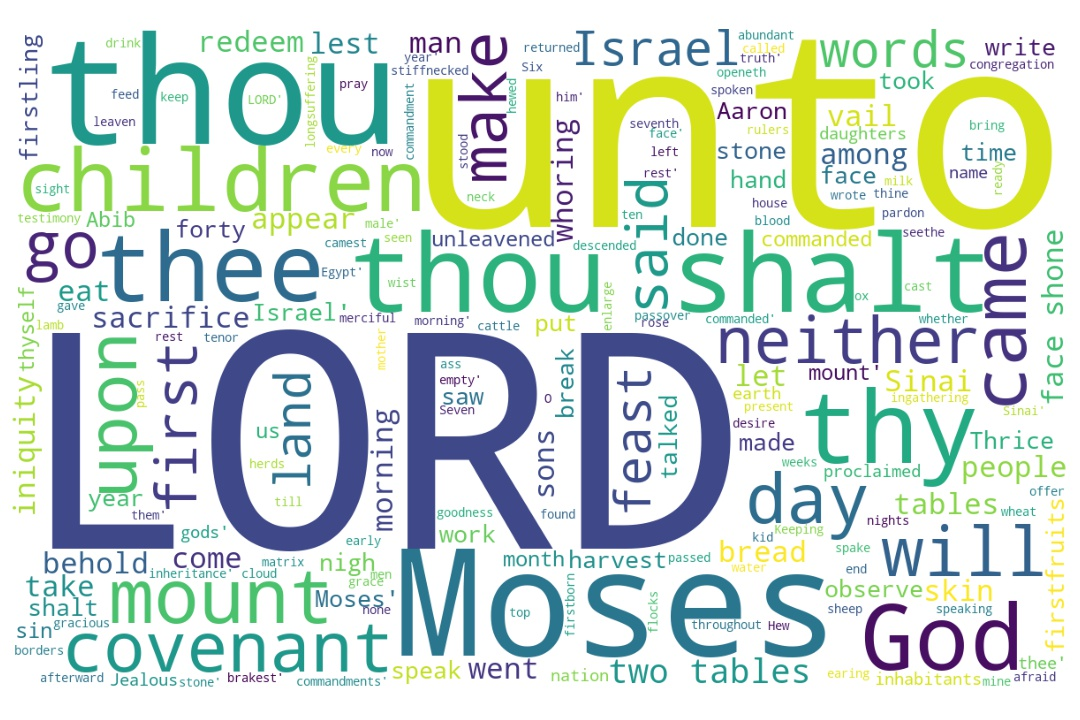
\includegraphics[width=\linewidth]{02OT-Exodus/Exodus34-WordCloud.jpg}
  \caption{Exodus 34 Word Cloud}
  \label{fig:Exodus 34 word Cloud}
\end{figure}



\marginpar{\scriptsize \centering \fcolorbox{bone}{lime}{\textbf{BE READY}}\\ (Exodus 34:1-35) \begin{compactenum}[I.][8]
    \item To \textbf{Receive Instruction} from God \index[scripture]{Exodus!Exo 34:02}(Exodus 34:2)
    \item To be \textbf{Visited} by God\index[scripture]{Exodus!Exo  19:11}(Exo 19:11)
    \item To be \textbf{Rescued} by God \index[scripture]{Esther!Est 08:13}(Est 8:13)
    \item For a \textbf{Revelation} \index[scripture]{Job!Job 18:12}(Job 18:12)
    \item To \textbf{Reject} False gods \index[scripture]{Daniel!Dan 03:15}(Dan 3:15)
    \item To \textbf{Render} Gifts \index[scripture]{2 Corinthians!2Cor 09:03}\index[scripture]{2 Corinthians!2 Corinthians 09:05}(2 Cor 9:3, 5)
   \item To \textbf{Respond} for God \index[scripture]{1 Peter!1Pet 03:15}(1 Pet 3:15)
%    \item A \textbf{Service} \index[scripture]{Exodus!Exodus 27:19}(Exodus 27:19)
%    \item A \textbf{Statute} \index[scripture]{Exodus!Exodus 27:21}(Exodus 27:21)
%    \item The \textbf{Sons} \index[scripture]{Exodus!Exodus 27:21}(Exodus 27:21)
\end{compactenum}}

%%%%%%%%%%%%%%%%%%%%%%%%%%%%%%%%%%%%%%
%%%%%%%%%%%%%%%%%%%%%%%%%%%%%%%%%%%%%
\footnote{\textcolor[cmyk]{0.99998,1,0,0}{\hyperlink{TOC}{Return to end of Table of Contents.}}}\footnote{\href{https://audiobible.com/bible/exodus_34.html}{\textcolor[cmyk]{0.99998,1,0,0}{Exodus 34 Audio}}}\textcolor[cmyk]{0.99998,1,0,0}{And the LORD said unto \fcolorbox{bone}{bone}{Moses}, Hew thee two tables of stone like unto the first: and I will write upon \emph{these} tables the words that were in the first tables, which thou brakest.}
[2] \textcolor[cmyk]{0.99998,1,0,0}{And \fcolorbox{bone}{lime}{be ready} in the morning, and come up in the morning unto mount Sinai, and present thyself there to me in the top of the mount.}
[3] \textcolor[cmyk]{0.99998,1,0,0}{And no man shall come up with thee, neither let any man be seen throughout all the mount; neither let the flocks nor herds feed before that mount.}\\
\\
\P \textcolor[cmyk]{0.99998,1,0,0}{And he hewed two tables of stone like unto the first; and \fcolorbox{bone}{bone}{Moses} rose up early in the morning, and went up unto mount Sinai, as the LORD had commanded him, and took in his hand the two tables of stone.}
[5] \textcolor[cmyk]{0.99998,1,0,0}{And the LORD descended in the cloud, and stood with him there, and proclaimed the name of the LORD.}
[6] \textcolor[cmyk]{0.99998,1,0,0}{And the LORD passed by before him, and proclaimed, The LORD, The LORD God, merciful and gracious, longsuffering, and abundant in goodness and truth,}
[7] \textcolor[cmyk]{0.99998,1,0,0}{Keeping mercy for thousands, forgiving iniquity and transgression and sin, and that will by no means clear \emph{the} \emph{guilty}; visiting the iniquity of the fathers upon the children, and upon the children's children, unto the third and to the fourth \emph{generation}.}
[8] \textcolor[cmyk]{0.99998,1,0,0}{And \fcolorbox{bone}{bone}{Moses} made haste, and bowed his head toward the earth, and worshipped.}
[9] \textcolor[cmyk]{0.99998,1,0,0}{And he said, If now I have found grace in thy sight, O Lord, let my Lord, I pray thee, go among us; for it \emph{is} a stiffnecked people; and pardon our iniquity and our sin, and take us for thine inheritance.}
[10] \textcolor[cmyk]{0.99998,1,0,0}{And he said, Behold, I make a covenant: before all thy people I will do marvels, such as have not been done in all the earth, nor in any nation: and all the people among which thou \emph{art} shall see the work of the LORD: for it \emph{is} a terrible thing that I will do with thee.}
[11] \textcolor[cmyk]{0.99998,1,0,0}{Observe thou that which I command thee \fcolorbox{bone}{lime}{this day}: behold, I drive out before thee the Amorite, and the Canaanite, and the Hittite, and the Perizzite, and the Hivite, and the Jebusite.}
[12] \textcolor[cmyk]{0.99998,1,0,0}{Take heed to thyself, lest thou make a covenant with the inhabitants of the land whither thou goest, lest it be for a snare in the midst of thee:}
[13] \textcolor[cmyk]{0.99998,1,0,0}{But ye shall destroy their altars, break their images, and cut down their groves:}
[14] \textcolor[cmyk]{0.99998,1,0,0}{For thou shalt worship no other god: for the LORD, whose name \emph{is} Jealous, \emph{is} a jealous God:}
[15] \textcolor[cmyk]{0.99998,1,0,0}{Lest thou make a covenant with the inhabitants of the land, and they go a whoring after their gods, and do sacrifice unto their gods, and \emph{one} call thee, and thou eat of his sacrifice;}
[16] \textcolor[cmyk]{0.99998,1,0,0}{And thou take of their daughters unto thy sons, and their daughters go a whoring after their gods, and make thy sons go a whoring after their gods.}
[17] \textcolor[cmyk]{0.99998,1,0,0}{Thou shalt make thee no molten gods.}\\
\\
\P \textcolor[cmyk]{0.99998,1,0,0}{The feast of unleavened bread shalt thou keep. Seven days thou shalt eat unleavened bread, as I commanded thee, in the time of the month Abib: for in the month Abib thou camest out from Egypt.}
[19] \textcolor[cmyk]{0.99998,1,0,0}{All that openeth the matrix \emph{is} mine; and every firstling among thy cattle, \emph{whether} ox or sheep, \emph{that} \emph{is} \emph{male}.}
[20] \textcolor[cmyk]{0.99998,1,0,0}{But the firstling of an ass thou shalt redeem with a lamb: and if thou redeem \emph{him} not, then shalt thou break his neck. All the firstborn of thy sons thou shalt redeem. And none shall appear before me empty.}\\
\\
\P \textcolor[cmyk]{0.99998,1,0,0}{Six days thou shalt work, but on the seventh day thou shalt rest: in earing time and in harvest thou shalt rest.}\\
\\
\P \textcolor[cmyk]{0.99998,1,0,0}{And thou shalt observe the feast of weeks, of the firstfruits of wheat harvest, and the feast of ingathering at the year's end.}\\
\\
\P \textcolor[cmyk]{0.99998,1,0,0}{Thrice in the year shall all your men children appear before the Lord GOD, the God of Israel.}
[24] \textcolor[cmyk]{0.99998,1,0,0}{For I will cast out the nations before thee, and enlarge thy borders: neither shall any man desire thy land, when thou shalt go up to appear before the LORD thy God thrice in the year.}
[25] \textcolor[cmyk]{0.99998,1,0,0}{Thou shalt not offer the blood of my sacrifice with leaven; neither shall the sacrifice of the feast of the passover be left unto the morning.}
[26] \textcolor[cmyk]{0.99998,1,0,0}{The first of the firstfruits of thy land thou shalt bring unto the house of the LORD thy God. Thou shalt not seethe a kid in his mother's milk.}
[27] \textcolor[cmyk]{0.99998,1,0,0}{And the LORD said unto \fcolorbox{bone}{bone}{Moses}, Write thou these words: for after the tenor of these words I have made a covenant with thee and with Israel.}
[28] \textcolor[cmyk]{0.99998,1,0,0}{And he was there with the LORD forty days and forty nights; he did neither eat bread, nor drink water. And he wrote upon the tables the words of the covenant, the ten commandments.}\\
\\
\P \textcolor[cmyk]{0.99998,1,0,0}{And it came to pass, when \fcolorbox{bone}{bone}{Moses} came down from mount Sinai with the two tables of testimony in Moses' hand, when he came down from the mount, that \fcolorbox{bone}{bone}{Moses} wist not that the skin of his face shone while he talked with him.}
[30] \textcolor[cmyk]{0.99998,1,0,0}{And when Aaron and all the children of Israel saw \fcolorbox{bone}{bone}{Moses}, behold, the skin of his face shone; and they were afraid to come nigh him.}
[31] \textcolor[cmyk]{0.99998,1,0,0}{And \fcolorbox{bone}{bone}{Moses} called unto them; and Aaron and all the rulers of the congregation returned unto him: and \fcolorbox{bone}{bone}{Moses} talked with them.}
[32] \textcolor[cmyk]{0.99998,1,0,0}{And afterward all the children of Israel came nigh: and he gave them in commandment all that the LORD had spoken with him in mount Sinai.}
[33] \textcolor[cmyk]{0.99998,1,0,0}{And \emph{till} \fcolorbox{bone}{bone}{Moses} had done speaking with them, he put a vail on his face.}
[34] \textcolor[cmyk]{0.99998,1,0,0}{But when \fcolorbox{bone}{bone}{Moses} went in before the LORD to speak with him, he took the vail off, until he came out. And he came out, and spake unto the children of Israel \emph{that} which he was commanded.}
[35] \textcolor[cmyk]{0.99998,1,0,0}{And the children of Israel saw the face of \fcolorbox{bone}{bone}{Moses}, that the skin of Moses' face shone: and \fcolorbox{bone}{bone}{Moses} put the vail upon his face again, until he went in to speak with him.}
\chapter{Exodus 35}


\begin{figure}
  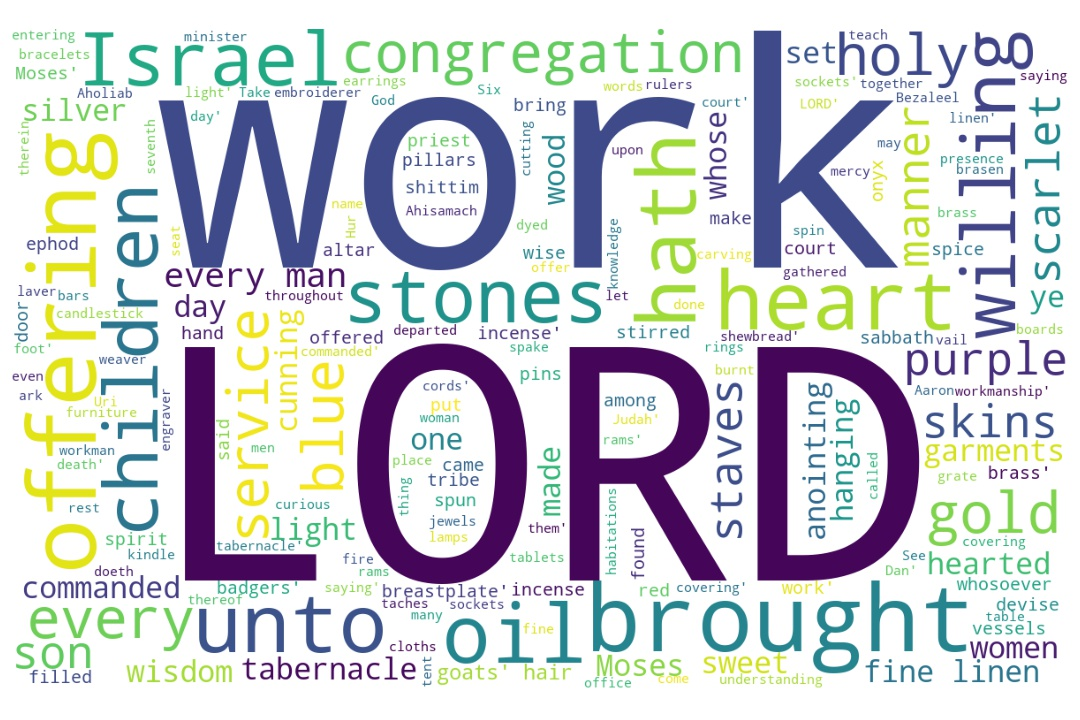
\includegraphics[width=\linewidth]{02OT-Exodus/Exodus35-WordCloud.jpg}
  \caption{Exodus 35 Word Cloud}
  \label{fig:Exodus 35 word Cloud}
\end{figure}


\marginpar{\scriptsize \centering \fcolorbox{bone}{lime}{\textbf{BUILDING A CHURCH}}\\ (Exodus 35:1-35) \begin{compactenum}[I.][8]
    \item A \textbf{Drawing} Together \index[scripture]{Exodus!Exo 35:01}(Exo 35:1)
    \item \textbf{Distinct} Rules \index[scripture]{Exodus!Exo 35:02}(Exo 35:2)
    \item \textbf{Devotion} \index[scripture]{Exodus!Exodus 35:05}(Exo 35:5)
    \item \textbf{Dedication} %\index[scripture]{Exodus!Exodus 35:02}(Exodus 35:2)
    \item A \textbf{Display} of Interest \& Involvment  \index[scripture]{Exodus!Exodus 35:10}(Exo 35:10)
    \item \textbf{Decisions} to be part of the effort %\index[scripture]{Exodus!Exodus 35:02}(Exo 35:2)
    \item \textbf{Departure} back into real life 
\end{compactenum}}










\footnote{\textcolor[cmyk]{0.99998,1,0,0}{\hyperlink{TOC}{Return to end of Table of Contents.}}}\footnote{\href{https://audiobible.com/bible/exodus_35.html}{\textcolor[cmyk]{0.99998,1,0,0}{Exodus 35 Audio}}}\textcolor[cmyk]{0.99998,1,0,0}{And Moses \fcolorbox{bone}{lime}{gathered}  \fcolorbox{bone}{bone}{all} the congregation of the children of Israel together, and said unto them, These \emph{are} the words which the LORD hath commanded, that \emph{ye} should do them.}
[2] \textcolor[cmyk]{0.99998,1,0,0}{Six days shall work be done, but on the seventh day \fcolorbox{bone}{lime}{there shall be} to you an holy day, a sabbath of rest to the LORD: whosoever doeth work therein shall be put to death.}
[3] \textcolor[cmyk]{0.99998,1,0,0}{Ye shall kindle no fire throughout your habitations upon the sabbath day.}\\
\\
\P \textcolor[cmyk]{0.99998,1,0,0}{And Moses spake unto  \fcolorbox{bone}{bone}{all} the congregation of the children of Israel, saying, This \emph{is} the thing which the LORD commanded, saying,}
[5] \textcolor[cmyk]{0.99998,1,0,0}{Take ye from among you an offering unto the LORD: whosoever \emph{is} of a \fcolorbox{bone}{lime}{willing heart}, let him bring it, an offering of the LORD; gold, and silver, and brass,}
[6] \textcolor[cmyk]{0.99998,1,0,0}{And blue, and purple, and scarlet, and fine linen, and goats' \emph{hair},}
[7] \textcolor[cmyk]{0.99998,1,0,0}{And rams' skins dyed red, and badgers' skins, and shittim wood,}
[8] \textcolor[cmyk]{0.99998,1,0,0}{And oil for the light, and spices for anointing oil, and for the sweet incense,}
[9] \textcolor[cmyk]{0.99998,1,0,0}{And onyx stones, and stones to be set for the ephod, and for the breastplate.}
[10] \textcolor[cmyk]{0.99998,1,0,0}{And every wise hearted among you shall come, and make  \fcolorbox{bone}{bone}{all} that the LORD hath commanded;}
[11] \textcolor[cmyk]{0.99998,1,0,0}{The tabernacle, his tent, and his covering, his taches, and his boards, his bars, his pillars, and his sockets,}
[12] \textcolor[cmyk]{0.99998,1,0,0}{The ark, and the staves thereof, \emph{with} the mercy seat, and the vail of the covering,}
[13] \textcolor[cmyk]{0.99998,1,0,0}{The table, and his staves, and  \fcolorbox{bone}{bone}{all} his vessels, and the shewbread,}
[14] \textcolor[cmyk]{0.99998,1,0,0}{The candlestick also for the light, and his furniture, and his lamps, with the oil for the light,}
[15] \textcolor[cmyk]{0.99998,1,0,0}{And the incense altar, and his staves, and the anointing oil, and the sweet incense, and the hanging for the door at the entering in of the tabernacle,}
[16] \textcolor[cmyk]{0.99998,1,0,0}{The altar of burnt offering, with his brasen grate, his staves, and  \fcolorbox{bone}{bone}{all} his vessels, the laver and his foot,}
[17] \textcolor[cmyk]{0.99998,1,0,0}{The hangings of the court, his pillars, and their sockets, and the hanging for the door of the court,}
[18] \textcolor[cmyk]{0.99998,1,0,0}{The pins of the tabernacle, and the pins of the court, and their cords,}
[19] \textcolor[cmyk]{0.99998,1,0,0}{The cloths of service, to do service in the holy \emph{place}, the holy garments for Aaron the priest, and the garments of his sons, to minister in the priest's office.}\\
\\
\P \textcolor[cmyk]{0.99998,1,0,0}{And  \fcolorbox{bone}{bone}{all} the congregation of the children of Israel departed from the presence of Moses.}
[21] \textcolor[cmyk]{0.99998,1,0,0}{And they came, every one whose heart stirred him up, and every one whom his spirit made willing, \emph{and} they brought the LORD'S offering to the work of the tabernacle of the congregation, and for  \fcolorbox{bone}{bone}{all} his service, and for the holy garments.}
[22] \textcolor[cmyk]{0.99998,1,0,0}{And they came, both men and women, as many as were willing hearted, \emph{and} brought bracelets, and earrings, and rings, and tablets,  \fcolorbox{bone}{bone}{all} jewels of gold: and every man that offered \emph{offered} an offering of gold unto the LORD.}
[23] \textcolor[cmyk]{0.99998,1,0,0}{And every man, with whom was found blue, and purple, and scarlet, and fine linen, and goats' \emph{hair}, and red skins of rams, and badgers' skins, brought \emph{them}.}
[24] \textcolor[cmyk]{0.99998,1,0,0}{Every one that did offer an offering of silver and brass brought the LORD'S offering: and every man, with whom was found shittim wood for any work of the service, brought \emph{it}.}
[25] \textcolor[cmyk]{0.99998,1,0,0}{And  \fcolorbox{bone}{bone}{all} the women that were wise hearted did spin with their hands, and brought that which they had spun, \emph{both} of blue, and of purple, \emph{and} of scarlet, and of fine linen.}
[26] \textcolor[cmyk]{0.99998,1,0,0}{And  \fcolorbox{bone}{bone}{all} the women whose heart stirred them up in wisdom spun goats' \emph{hair}.}
[27] \textcolor[cmyk]{0.99998,1,0,0}{And the rulers brought onyx stones, and stones to be set, for the ephod, and for the breastplate;}
[28] \textcolor[cmyk]{0.99998,1,0,0}{And spice, and oil for the light, and for the anointing oil, and for the sweet incense.}
[29] \textcolor[cmyk]{0.99998,1,0,0}{The children of Israel brought a willing offering unto the LORD, every man and woman, whose heart made them willing to bring for  \fcolorbox{bone}{bone}{all} manner of work, which the LORD had commanded to be made by the hand of Moses.}\\
\\
\P \textcolor[cmyk]{0.99998,1,0,0}{And Moses said unto the children of Israel, See, the LORD hath called by name Bezaleel the son of Uri, the son of Hur, of the tribe of Judah;}
[31] \textcolor[cmyk]{0.99998,1,0,0}{And he hath filled him with the spirit of God, in wisdom, in understanding, and in knowledge, and in  \fcolorbox{bone}{bone}{all} manner of workmanship;}
[32] \textcolor[cmyk]{0.99998,1,0,0}{And to devise curious works, to work in gold, and in silver, and in brass,}
[33] \textcolor[cmyk]{0.99998,1,0,0}{And in the cutting of stones, to set \emph{them}, and in carving of wood, to make any manner of cunning work.}
[34] \textcolor[cmyk]{0.99998,1,0,0}{And he hath put in his heart that he may teach, \emph{both} he, and Aholiab, the son of Ahisamach, of the tribe of Dan.}
[35] \textcolor[cmyk]{0.99998,1,0,0}{Them hath he filled with wisdom of heart, to work  \fcolorbox{bone}{bone}{all} manner of work, of the engraver, and of the cunning workman, and of the embroiderer, in blue, and in purple, in scarlet, and in fine linen, and of the weaver, \emph{even} of them that do any work, and of those that devise cunning work.}
\chapter{Exodus 36}

\begin{figure}
  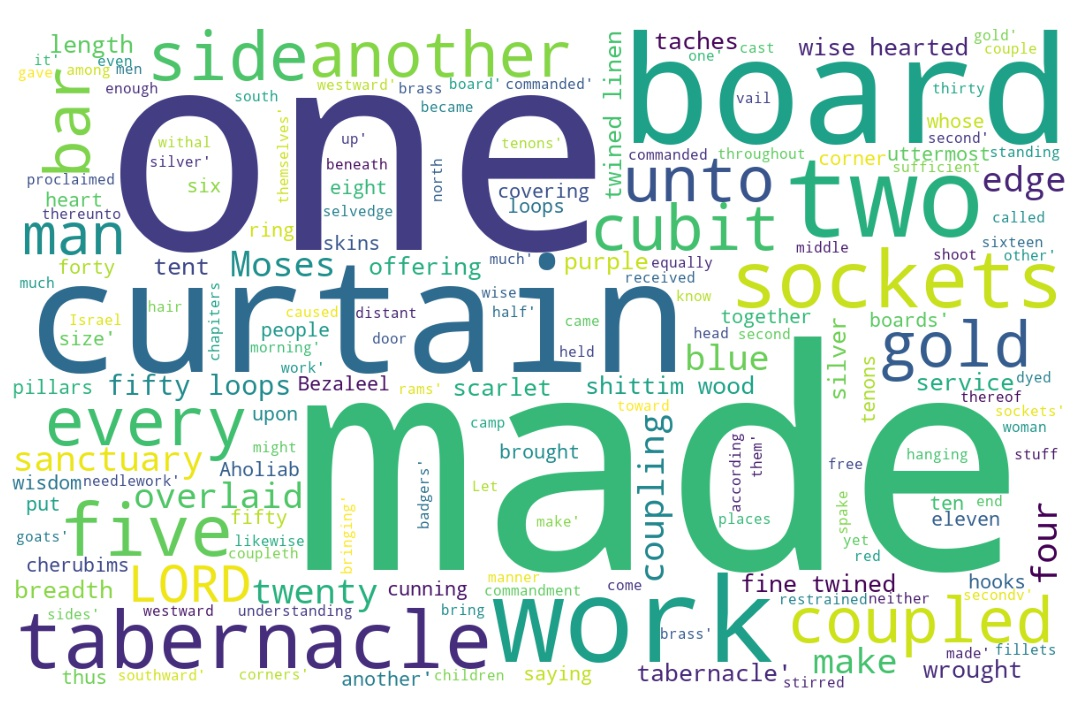
\includegraphics[width=\linewidth]{02OT-Exodus/Exodus36-WordCloud.jpg}
  \caption{Exodus 36 Word Cloud}
  \label{fig:Exodus 36 word Cloud}
\end{figure}

\marginpar{\scriptsize \centering \fcolorbox{bone}{lime}{\textbf{DOING THE WORK}}\\ (Exodus 36:1-38) \begin{compactenum}[I.][8]
    \item An \textbf{Enlightened} Group \index[scripture]{Exodus!Exo 36:01}\index[scripture]{Exodus!Exo 36:02}(Exo 36:1, 2)
    \item \textbf{Envisioned Goal} \index[scripture]{Exodus!Exo 36:02}(Exo 36:2)
    \item \textbf{Excess Giving} \index[scripture]{Exodus!Exo 36:05}(Exo 36:5)
    \item \textbf{Exhibited Grace} \index[scripture]{Exodus!Exo 36:06}(Exo 36:6) 
    \item \textbf{Echoed Guidance} \index[scripture]{Exodus!Exo 36:08-38}(Exo 36:8--38) (repeated for Exodus 26:1--37)
    \item \textbf{Employed Gold} \index[scripture]{Exodus!Exo 36:34}\index[scripture]{Exodus!Exo 36:36}(Exo 36:34, 36)
\end{compactenum}}










\footnote{\textcolor[cmyk]{0.99998,1,0,0}{\hyperlink{TOC}{Return to end of Table of Contents.}}}\footnote{\href{https://audiobible.com/bible/exodus_36.html}{\textcolor[cmyk]{0.99998,1,0,0}{Exodus 36 Audio}}}\textcolor[cmyk]{0.99998,1,0,0}{Then wrought Bezaleel and Aholiab, and every wise hearted man, in whom \fcolorbox{bone}{lime}{the LORD put wisdom and understanding} to know how to work all manner of work for the service of the sanctuary, according to all that the LORD had commanded.}
[2] \textcolor[cmyk]{0.99998,1,0,0}{And Moses called Bezaleel and Aholiab, and every wise hearted man, in whose heart the LORD \fcolorbox{bone}{lime}{had put wisdom}, \emph{even} every one whose heart \fcolorbox{bone}{lime}{stirred} him up to come unto the work to do it:}
[3] \textcolor[cmyk]{0.99998,1,0,0}{And they received of Moses all the offering, which the children of Israel had brought for the work of the service of the sanctuary, to make it \emph{withal}. And they brought yet unto him free offerings every morning.}
[4] \textcolor[cmyk]{0.99998,1,0,0}{And all the wise men, that wrought all the work of the sanctuary, came every man from his work which they made;}\\
\\
\P \textcolor[cmyk]{0.99998,1,0,0}{And they spake unto Moses, saying, The people bring much \fcolorbox{bone}{lime}{more than} \fcolorbox{bone}{lime}{enough} for the service of the work, which the LORD commanded to make.}
[6] \textcolor[cmyk]{0.99998,1,0,0}{And Moses gave commandment, and they caused it to be proclaimed throughout the camp, saying, Let neither man nor woman make any more work for the offering of the sanctuary. So the people were \fcolorbox{bone}{lime}{restrained} from bringing.}
[7] \textcolor[cmyk]{0.99998,1,0,0}{For the stuff they had was sufficient for all the work to make it, and too much.}\\
\\
\P \textcolor[cmyk]{0.99998,1,0,0}{And every wise hearted man among them that wrought the work of the \fcolorbox{bone}{bone}{tabernacle} made ten curtains \emph{of} fine twined linen, and blue, and purple, and scarlet: \emph{with} cherubims of cunning work made he them.}
[9] \textcolor[cmyk]{0.99998,1,0,0}{The length of one curtain \emph{was} twenty and eight cubits, and the breadth of one curtain four cubits: the curtains \emph{were} all of one size.}
[10] \textcolor[cmyk]{0.99998,1,0,0}{And he coupled the five curtains one unto another: and \emph{the} \emph{other} five curtains he coupled one unto another.}
[11] \textcolor[cmyk]{0.99998,1,0,0}{\fcolorbox{bone}{bone}{And he made} loops of blue on the edge of one curtain from the selvedge in the coupling: likewise he made in the uttermost side of \emph{another} curtain, in the coupling of the second.}
[12] \textcolor[cmyk]{0.99998,1,0,0}{Fifty loops made he in one curtain, and fifty loops made he in the edge of the curtain which \emph{was} in the coupling of the second: the loops held one \emph{curtain} to another.}
[13] \textcolor[cmyk]{0.99998,1,0,0}{\fcolorbox{bone}{bone}{And he made} fifty taches of gold, and coupled the curtains one unto another with the taches: so it became one \fcolorbox{bone}{bone}{tabernacle}.}\\
\\
\P \textcolor[cmyk]{0.99998,1,0,0}{\fcolorbox{bone}{bone}{And he made} curtains \emph{of} goats' \emph{hair} for the tent over the \fcolorbox{bone}{bone}{tabernacle}: eleven curtains he made them.}
[15] \textcolor[cmyk]{0.99998,1,0,0}{The length of one curtain \emph{was} thirty cubits, and four cubits \emph{was} the breadth of one curtain: the eleven curtains \emph{were} of one size.}
[16] \textcolor[cmyk]{0.99998,1,0,0}{And he coupled five curtains by themselves, and six curtains by themselves.}
[17] \textcolor[cmyk]{0.99998,1,0,0}{\fcolorbox{bone}{bone}{And he made} fifty loops upon the uttermost edge of the curtain in the coupling, and fifty loops made he upon the edge of the curtain which coupleth the second.}
[18] \textcolor[cmyk]{0.99998,1,0,0}{\fcolorbox{bone}{bone}{And he made} fifty taches \emph{of} brass to couple the tent together, that it might be one.}
[19] \textcolor[cmyk]{0.99998,1,0,0}{\fcolorbox{bone}{bone}{And he made} a covering for the tent \emph{of} rams' skins dyed red, and a covering \emph{of} badgers' skins above \emph{that}.}\\
\\
\P \textcolor[cmyk]{0.99998,1,0,0}{\fcolorbox{bone}{bone}{And he made} boards for the \fcolorbox{bone}{bone}{tabernacle} \emph{of} shittim wood, standing up.}
[21] \textcolor[cmyk]{0.99998,1,0,0}{The length of a board \emph{was} ten cubits, and the breadth of a board one cubit and a half.}
[22] \textcolor[cmyk]{0.99998,1,0,0}{One board had two tenons, equally distant one from another: thus did he make for all the boards of the \fcolorbox{bone}{bone}{tabernacle}.}
[23] \textcolor[cmyk]{0.99998,1,0,0}{\fcolorbox{bone}{bone}{And he made} boards for the \fcolorbox{bone}{bone}{tabernacle}; twenty boards for the south side southward:}
[24] \textcolor[cmyk]{0.99998,1,0,0}{And forty sockets of silver he made under the twenty boards; two sockets under one board for his two tenons, and two sockets under another board for his two tenons.}
[25] \textcolor[cmyk]{0.99998,1,0,0}{And for the other side of the \fcolorbox{bone}{bone}{tabernacle}, \emph{which} \emph{is} toward the north corner, he made twenty boards,}
[26] \textcolor[cmyk]{0.99998,1,0,0}{And their forty sockets of silver; two sockets under one board, and two sockets under another board.}
[27] \textcolor[cmyk]{0.99998,1,0,0}{And for the sides of the \fcolorbox{bone}{bone}{tabernacle} westward he made six boards.}
[28] \textcolor[cmyk]{0.99998,1,0,0}{And two boards made he for the corners of the \fcolorbox{bone}{bone}{tabernacle} in the two sides.}
[29] \textcolor[cmyk]{0.99998,1,0,0}{And they were coupled beneath, and coupled together at the head thereof, to one ring: thus he did to both of them in both the corners.}
[30] \textcolor[cmyk]{0.99998,1,0,0}{And there were eight boards; and their sockets \emph{were} sixteen sockets of silver, under every board two sockets.}\\
\\
\P \textcolor[cmyk]{0.99998,1,0,0}{\fcolorbox{bone}{bone}{And he made} bars of shittim wood; five for the boards of the one side of the \fcolorbox{bone}{bone}{tabernacle},}
[32] \textcolor[cmyk]{0.99998,1,0,0}{And five bars for the boards of the other side of the \fcolorbox{bone}{bone}{tabernacle}, and five bars for the boards of the \fcolorbox{bone}{bone}{tabernacle} for the sides westward.}
[33] \textcolor[cmyk]{0.99998,1,0,0}{\fcolorbox{bone}{bone}{And he made} the middle bar to shoot through the boards from the one end to the other.}
[34] \textcolor[cmyk]{0.99998,1,0,0}{And he overlaid the boards with \fcolorbox{bone}{lime}{gold}, and made their rings \emph{of} gold \emph{to} \emph{be} places for the bars, and overlaid the bars with \fcolorbox{bone}{lime}{gold}.}\\
\\
\P \textcolor[cmyk]{0.99998,1,0,0}{\fcolorbox{bone}{bone}{And he made} a vail \emph{of} blue, and purple, and scarlet, and fine twined linen: \emph{with} cherubims made he it of cunning work.}
[36] \textcolor[cmyk]{0.99998,1,0,0}{\fcolorbox{bone}{bone}{And he made} thereunto four pillars \emph{of} shittim \emph{wood}, and overlaid them with gold: their hooks \emph{were} \emph{of} \fcolorbox{bone}{lime}{gold}; and he cast for them four sockets of silver.}\\
\\
\P \textcolor[cmyk]{0.99998,1,0,0}{\fcolorbox{bone}{bone}{And he made} an hanging for the \fcolorbox{bone}{bone}{tabernacle} door \emph{of} blue, and purple, and scarlet, and fine twined linen, of needlework;}
[38] \textcolor[cmyk]{0.99998,1,0,0}{And the five pillars of it with their hooks: and he overlaid their chapiters and their fillets with gold: but their five sockets \emph{were} \emph{of} brass.}

\chapter{Psalm 29}

\begin{figure}
  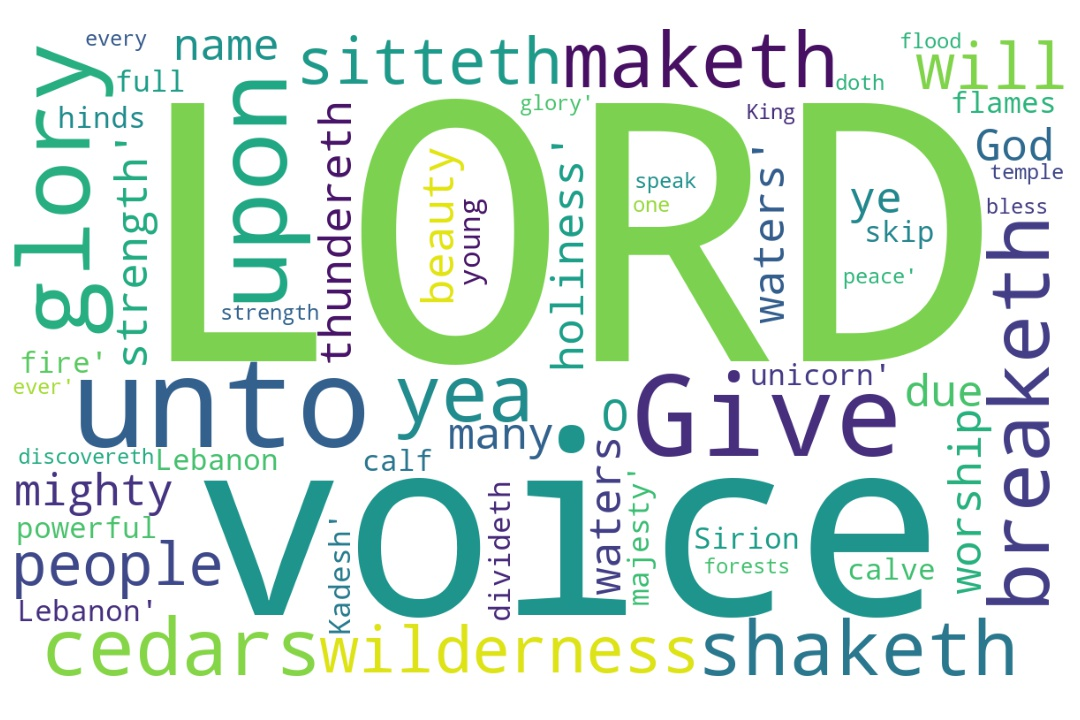
\includegraphics[width=\linewidth]{19OT-Psalms/Psalm29-WordCloud.jpg}
  \caption{Psalm 29 Word Cloud}
  \label{fig:Psalm 29 word Cloud}
\end{figure}


\marginpar{\scriptsize \centering \fcolorbox{bone}{lime}{\textbf{THE VOICE OF THE LORD}}\\ (Psalm 29:1-11) \begin{compactenum}[I.][8]
    \item \textbf{God's Place} \index[scripture]{Psalms!Psa 029:01}(Psa 29:1)
    \item \textbf{God's Presence Obvious} \index[scripture]{Psalms!Psa 029:03-09}(Psa 29:3-9)
    \item \textbf{God's Power Observed} \index[scripture]{Psalms!Psa 029:04}(Psa 29:4)
    \item \textbf{God's Peace Obtained} \index[scripture]{Psalms!Psa 029:11}(Psa 29:11)
    \item \textbf{God's People} \index[scripture]{Psalms!Psa 029:11}(Psa 29:11)
    \item \textbf{God's Preservation Ordained} \index[scripture]{Psalms!Psa 029:11}(Psa 29:11)
    \item \textbf{God's Providence}
\end{compactenum}}

\footnote{\textcolor[cmyk]{0.99998,1,0,0}{\hyperlink{TOC}{Return to end of Table of Contents.}}}\footnote{\href{https://www.audioverse.org/english/audiobibles/books/ENGKJV/O/Ps/1}{\textcolor[cmyk]{0.99998,1,0,0}{Psalms Audio}}}\textcolor[cmyk]{0.99998,1,0,0}{Give unto the LORD, O ye mighty, \fcolorbox{bone}{lime}{give unto the LORD} glory and strength.}
[2] \textcolor[cmyk]{0.99998,1,0,0}{Give unto the LORD the glory due unto his name; worship the LORD in the beauty of holiness.}
[3] \textcolor[cmyk]{0.99998,1,0,0}{The voice of the LORD \emph{is} upon the waters: the God of glory \fcolorbox{bone}{lime}{thundereth}: the LORD \emph{is} upon many waters.}
[4] \textcolor[cmyk]{0.99998,1,0,0}{The voice of the LORD \emph{is} \fcolorbox{bone}{lime}{powerful}; the voice of the LORD \emph{is} full of majesty.}
[5] \textcolor[cmyk]{0.99998,1,0,0}{The voice of the LORD breaketh the cedars; yea, the LORD breaketh the cedars of Lebanon.}
[6] \textcolor[cmyk]{0.99998,1,0,0}{He maketh them also to skip like a calf; Lebanon and Sirion like a young unicorn.}
[7] \textcolor[cmyk]{0.99998,1,0,0}{The voice of the LORD divideth the flames of fire.}
[8] \textcolor[cmyk]{0.99998,1,0,0}{The voice of the LORD shaketh the wilderness; the LORD shaketh the wilderness of Kadesh.}
[9] \textcolor[cmyk]{0.99998,1,0,0}{The voice of the LORD maketh the hinds to calve, and discovereth the forests: and in his temple doth every one speak of \emph{his} glory.}
[10] \textcolor[cmyk]{0.99998,1,0,0}{The LORD sitteth upon the flood; yea, the LORD sitteth King for ever.}
[11] \textcolor[cmyk]{0.99998,1,0,0}{The LORD will give strength unto his \fcolorbox{bone}{lime}{people}; the LORD will bless his people with \fcolorbox{bone}{lime}{peace}.}



\
\chapter{Proverb 29}

\begin{figure}
  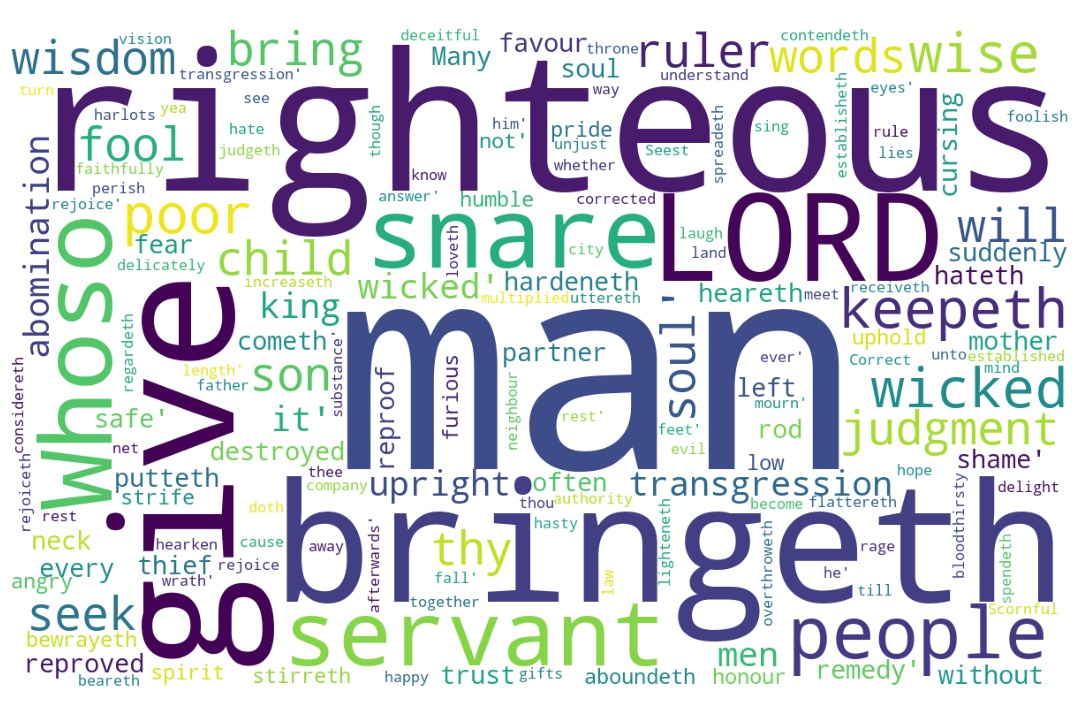
\includegraphics[width=\linewidth]{20OT-Proverbs/Proverb29-WordCloud.jpg}
  \caption{Proverb 29 Word Cloud}
  \label{fig:Proverb 29 word Cloud}
\end{figure}

\marginpar{\scriptsize \centering \fcolorbox{bone}{lime}{\textbf{MISSING WITHOUT WISDOM}}\\ (Proverb 29:1--27) 
\begin{compactenum}[I.][8]
    \item No \textbf{Remedy} \index[scripture]{Proverbs!Pro 29:01}(Pro 29:1) 
    \item No \textbf{Remorse} \index[scripture]{Proverbs!Pro 29:02}(Pro 29:2) 
    \item No \textbf{Rejoicing} \index[scripture]{Proverbs!Pro 29:06}(Pro 29:6) 
    \item No \textbf{Regard} \index[scripture]{Proverbs!Pro 29:07}(Pro 29:7) 
    \item No \textbf{Rest} \index[scripture]{Proverbs!Pro 29:09}(Pro 29:9) 
    \item No \textbf{Reproof} \index[scripture]{Proverbs!Pro 29:15}(Pro 29:15) 
    \item No \textbf{Restraint} \index[scripture]{Proverbs!Pro 29:16}(Pro 29:16) 
\end{compactenum} }

\footnote{\textcolor[cmyk]{0.99998,1,0,0}{\hyperlink{TOC}{Return to end of Table of Contents.}}}\footnote{\href{https://www.audioverse.org/english/audiobibles/books/ENGKJV/O/Prov/1}{\textcolor[cmyk]{0.99998,1,0,0}{Proverbs Audio}}}\textcolor[cmyk]{0.99998,1,0,0}{He, that being often reproved hardeneth \fcolorbox{bone}{bone}{his} neck, shall suddenly be destroyed, and that without \fcolorbox{bone}{lime}{remedy}.}
[2] \textcolor[cmyk]{0.99998,1,0,0}{When the righteous are in authority, the people rejoice: \fcolorbox{bone}{bone}{but} when the wicked beareth rule, the people \fcolorbox{bone}{lime}{mourn}.}
[3] \textcolor[cmyk]{0.99998,1,0,0}{Whoso loveth wisdom rejoiceth \fcolorbox{bone}{bone}{his} father: \fcolorbox{bone}{bone}{but} he that keepeth company with harlots spendeth \emph{his} substance.}
[4] \textcolor[cmyk]{0.99998,1,0,0}{The king by judgment establisheth the land: \fcolorbox{bone}{bone}{but} he that receiveth gifts overthroweth it.}
[5] \textcolor[cmyk]{0.99998,1,0,0}{A man that flattereth \fcolorbox{bone}{bone}{his} neighbour spreadeth a net for \fcolorbox{bone}{bone}{his} feet.}
[6] \textcolor[cmyk]{0.99998,1,0,0}{In the transgression of an evil man \emph{there} \emph{is} a snare: \fcolorbox{bone}{bone}{but} the righteous doth sing and \fcolorbox{bone}{lime}{rejoice}.}
[7] \textcolor[cmyk]{0.99998,1,0,0}{The righteous considereth the cause of the poor: \emph{but} the wicked \fcolorbox{bone}{lime}{regardeth} not to know \emph{it}.}
[8] \textcolor[cmyk]{0.99998,1,0,0}{Scornful men bring a city into a snare: \fcolorbox{bone}{bone}{but} wise \emph{men} turn away wrath.}
[9] \textcolor[cmyk]{0.99998,1,0,0}{\emph{If} a wise man contendeth with a foolish man, whether he rage or laugh, \emph{there} \emph{is} no \fcolorbox{bone}{lime}{rest}.}
[10] \textcolor[cmyk]{0.99998,1,0,0}{The bloodthirsty hate the upright: \fcolorbox{bone}{bone}{but} the just seek \fcolorbox{bone}{bone}{his} soul.}
[11] \textcolor[cmyk]{0.99998,1,0,0}{A fool uttereth all \fcolorbox{bone}{bone}{his} mind: \fcolorbox{bone}{bone}{but} a wise \emph{man} keepeth it in till afterwards.}
[12] \textcolor[cmyk]{0.99998,1,0,0}{If a ruler hearken to lies, all \fcolorbox{bone}{bone}{his} servants \emph{are} wicked.}
[13] \textcolor[cmyk]{0.99998,1,0,0}{The poor and the deceitful man meet together: the LORD lighteneth both their eyes.}
[14] \textcolor[cmyk]{0.99998,1,0,0}{The king that faithfully judgeth the poor, \fcolorbox{bone}{bone}{his} throne shall be established for ever.}
[15] \textcolor[cmyk]{0.99998,1,0,0}{The rod and \fcolorbox{bone}{lime}{reproof} give wisdom: \fcolorbox{bone}{bone}{but} a child left \emph{to} \emph{himself} bringeth \fcolorbox{bone}{bone}{his} mother to shame.}
[16] \textcolor[cmyk]{0.99998,1,0,0}{When the wicked are multiplied, \fcolorbox{bone}{lime}{\fcolorbox{bone}{MYGOLD}{transgression} increaseth}: \fcolorbox{bone}{bone}{but} the righteous shall see their fall.}
[17] \textcolor[cmyk]{0.99998,1,0,0}{Correct thy son, and he shall give thee rest; yea, he shall give delight unto thy soul.}
[18] \textcolor[cmyk]{0.99998,1,0,0}{Where \emph{there} \emph{is} no vision, the people perish: \fcolorbox{bone}{bone}{but} he that keepeth the law, happy \emph{is} he.}
[19] \textcolor[cmyk]{0.99998,1,0,0}{A servant will not be corrected by words: for though he understand he will not answer.}
[20] \textcolor[cmyk]{0.99998,1,0,0}{Seest thou a man \emph{that} \emph{is} hasty in \fcolorbox{bone}{bone}{his} words? \emph{there} \emph{is} more hope of a fool than of him.}
[21] \textcolor[cmyk]{0.99998,1,0,0}{He that delicately bringeth up \fcolorbox{bone}{bone}{his} servant from a child shall have him become \emph{his} son at the length.}
[22] \textcolor[cmyk]{0.99998,1,0,0}{An angry man stirreth up strife, and a furious man aboundeth in transgression.}
[23] \textcolor[cmyk]{0.99998,1,0,0}{A man's pride shall bring him low: \fcolorbox{bone}{bone}{but} honour shall uphold the humble in spirit.}
[24] \textcolor[cmyk]{0.99998,1,0,0}{Whoso is partner with a thief hateth \fcolorbox{bone}{bone}{his} own soul: he heareth cursing, and bewrayeth \emph{it} not.}
[25] \textcolor[cmyk]{0.99998,1,0,0}{The fear of man bringeth a snare: \fcolorbox{bone}{bone}{but} whoso putteth \fcolorbox{bone}{bone}{his} trust in the LORD shall be safe.}
[26] \textcolor[cmyk]{0.99998,1,0,0}{Many seek the ruler's favour; \fcolorbox{bone}{bone}{but} \emph{every} man's judgment \emph{cometh} from the LORD.}
[27] \textcolor[cmyk]{0.99998,1,0,0}{An unjust man \emph{is} an abomination to the just: and \emph{he} \emph{that} \emph{is} upright in the way \emph{is} abomination to the wicked.}




\end{document}

